\documentclass[a4paper,12pt]{article}

%Мои доработки
\usepackage[margin=10pt,font=small,labelfont=bf,
labelsep=period]{caption} % позволяет центровать подписи и издеваться над caption
%\usepackage{float} %здесь здесь, только здесь
\usepackage{floatrow} %нельзя одновременно включать floatrow и float
\usepackage{graphicx} %два пакета для размещения картинки и таблицы в ряд
%%% Работа с русским языком
\usepackage{enumitem} % развлекаться со списками
% объявляем новую команду для переноса строки внутри ячейки таблицы
\newcommand{\specialcell}[2][c]{%
	\begin{tabular}[#1]{@{}c@{}}#2\end{tabular}}
%	\renewcommand{\arraystretch}{1.8} %% increase table row spacing
%	\renewcommand{\tabcolsep}{1cm}   %% increase table column spacing


\usepackage{cmap}					% поиск в PDF
\usepackage{mathtext} 				% русские буквы в формулах
\usepackage[T2A]{fontenc}			% кодировка
\usepackage[utf8]{inputenc}			% кодировка исходного текста
\usepackage[english,russian]{babel}	% локализация и переносы

%%% Дополнительная работа с математикой
\usepackage{amsmath,amsfonts,amssymb,amsthm,mathtools} % AMS
\usepackage{icomma} % "Умная" запятая: $0,2$ --- число, $0, 2$ --- перечисление

%% Номера формул
%\mathtoolsset{showonlyrefs=true} % Показывать номера только у тех формул, на которые есть \eqref{} в тексте.
%\usepackage{leqno} % Нумерация формул слева

%% Свои команды
\DeclareMathOperator{\sgn}{\mathop{sgn}}

%% Перенос знаков в формулах (по Львовскому)
\newcommand*{\hm}[1]{#1\nobreak\discretionary{}
	{\hbox{$\mathsurround=0pt #1$}}{}}

%%% Работа с картинками
\usepackage{graphicx}  % Для вставки рисунков
\graphicspath{{images/}{images2/}}  % папки с картинками
\setlength\fboxsep{3pt} % Отступ рамки \fbox{} от рисунка
\setlength\fboxrule{1pt} % Толщина линий рамки \fbox{}
\usepackage{wrapfig} % Обтекание рисунков текстом

%%% Работа с таблицами
\usepackage{array,tabularx,tabulary,booktabs} % Дополнительная работа с таблицами
\usepackage{longtable}  % Длинные таблицы
\usepackage{multirow} % Слияние строк в таблице

%%% Теоремы
\theoremstyle{plain} % Это стиль по умолчанию, его можно не переопределять.
\newtheorem{theorem}{Теорема}[section]
\newtheorem{proposition}[theorem]{Утверждение}

\theoremstyle{definition} % "Определение"
\newtheorem{corollary}{Следствие}[theorem]
\newtheorem{problem}{Задача}[section]

\theoremstyle{remark} % "Примечание"
\newtheorem*{nonum}{Решение}

%%% Программирование
\usepackage{etoolbox} % логические операторы

%%% Страница
\usepackage{extsizes} % Возможность сделать 14-й шрифт
\usepackage{geometry} % Простой способ задавать поля
\geometry{top=25mm}
\geometry{bottom=35mm}
\geometry{left=35mm}
\geometry{right=20mm}
%

\usepackage{fancyhdr} % Колонтитулы
\pagestyle{fancy}
\renewcommand{\sectionmark}[1]{\markboth{#1}{}}
%\renewcommand{\headrulewidth}{0mm}  % Толщина линейки, отчеркивающей верхний колонтитул
%\lfoot{Нижний левый}
%\rfoot{Нижний правый}
%\rhead{}
%\chead{Верхний в центре}
\lhead{\thepage}
\cfoot{} % По умолчанию здесь номер страницы

\usepackage{setspace} % Интерлиньяж
%\onehalfspacing % Интерлиньяж 1.5
%\doublespacing % Интерлиньяж 2
%\singlespacing % Интерлиньяж 1

\usepackage{lastpage} % Узнать, сколько всего страниц в документе.

\usepackage{soul} % Модификаторы начертания

\usepackage{indentfirst} % Красная строка

\usepackage{soulutf8} % Модификаторы начертания

%\usepackage{hyperref}
%\usepackage[usenames,dvipsnames,svgnames,table,rgb]{xcolor}
%\hypersetup{				% Гиперссылки
%	unicode=true,           % русские буквы в раздела PDF
%	pdftitle={Заголовок},   % Заголовок
%	pdfsubject={Тема},      % Тема
%	pdfcreator={Создатель}, % Создатель
%	pdfproducer={Производитель}, % Производитель
%	pdfkeywords={keyword1} {key2} {key3}, % Ключевые слова
%	colorlinks=true,       	% false: ссылки в рамках; true: цветные ссылки
%	linkcolor=red,          % внутренние ссылки
%	citecolor=green,        % на библиографию
%	filecolor=magenta,      % на файлы
%	urlcolor=cyan           % на URL
%}

%\renewcommand{\familydefault}{\sfdefault} % Начертание шрифта


\usepackage{multicol} % Несколько колонок

\author{\LaTeX{} в Вышке}
\title{3.2 Оформление документа в целом}
\date{\today}

\begin{document} % конец преамбулы, начало документа
	\thispagestyle{empty}
	\begin{center}
		\textit{Федеральное государственное автономное образовательное\\ учреждение высшего образования }
		\vspace{0.5ex}
		
		\textbf{«Московский физико-технический институт\\ (национальный исследовательский университет)»}
	\end{center}
	\vspace{10ex}
	%\begin{flushright}
	%	\noindent
	%	\textit{Фамилия Имя Отчество}
	%	\\
	%	\textit{студент факультета экономики \\(группа 211И)}
	%\end{flushright}
	\begin{center}
		\vspace{13ex}
		\so{\textbf{Лабораторная работа №2.3.1Б}}
		\vspace{1ex}
		
		по курсу общей физики
		
		
		на тему:
		
		\textbf{\textit{<<Современные средства \\ получения и измерения вакуума>>}}
		\vspace{30ex}
		\begin{flushright}
			\noindent
			\textit{Работу выполнил:}
			\\
			\textit{Баринов Леонид \\(группа Б02-827)}
		\end{flushright}
		\vfill
		Долгопрудный \\2019
	\end{center}
	\newpage
	\setcounter{page}{1}
	\fancyhead[R]{\nouppercase{\leftmark}}
	\section{Аннотация}
	В работе будет определен:
	\begin{enumerate}
		\item Польный объем установки, высоковакуумной части, форвакуумной магистрали и самого насоса TMH. 
		\item Уровень течей по ухудшению вакуума после перекрытия откачки насосом TMH
	\end{enumerate} 
	
	Будет проведена оценка:
	\begin{enumerate}
		\item Эффективной скорости откачки системы форвакуумным насосом в области, где она почти постоянна в разных условиях: по схеме <<байпас>>, через диафрагмы $5\ \text{мм}$ и $1\ \text{мм}$, через фланец насоса TMH
		\item Эффективной скорости откачки системы турбомолекулярным насосом в области, где она почти постоянна в разных условиях: через фланец насоса TMH, через диафрагмы $10\ \text{мм}$ и $3 \ \text{мм}$
		\item Числа Кнудсена для предельных давлений при форвакуумной и высоковакуумной откачке в разных частях системы
	\end{enumerate}
	\section {Теоретические сведения}
	\subsection {Вакуум}
	В физике \textit{вакуумом} называют состояние газа, при котором характерная длина свободного пробега молекул в газе $\lambda$ сравнима по порядку величины с характерным линейным размером сосуда $d$, в котором газ находится. 
	
	В технике \textit{вакуумом} называют состояние газа при котором его давление меньше атмосферного $(Р < Р_\text{атм})$. Различают следующие типы вакуума: 
	\begin{itemize}
		\item Низкий, когда средняя длина свободного пробега молекул газа значительно меньше характерного линейного размера рассматриваемого объёма, т.е. \mbox{$\lambda < d$}
		\item Средний, когда $\lambda \sim d$
		\item  Высокий (или глубокий), когда $\lambda \gg d$
		\item Сверхвысокий вакуум, при котором не происходит заметного изменения свойств поверхности, первоначально свободной от адсорбированного газа, за время, существенное для проведения эксперимента. Газ в состоянии высокого вакуума называется ультраразреженным.
	\end{itemize}
\subsection{Некоторые понятия для работы с вакуумной техникой}
Основы процесса откачки и связанные с ним понятия рассмотрим на примере простейшей вакуумной системы (рис. 1)
\begin{figure}[H]
	\begin{center}
	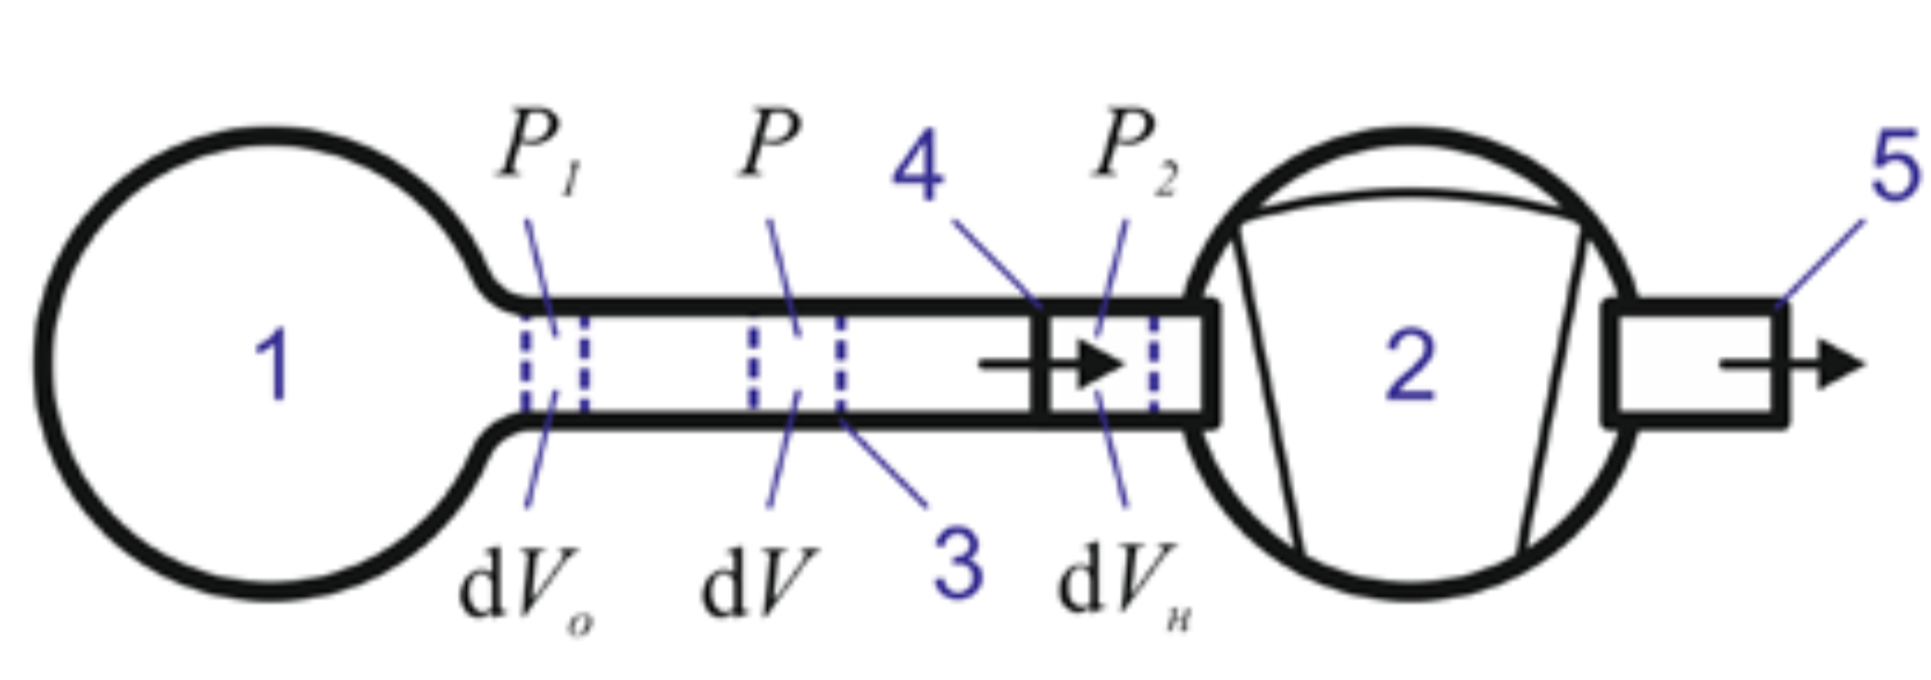
\includegraphics[width=0.6\linewidth]{1}
	\begin{tabular}{p{0.4\linewidth} p{0.4\linewidth}}
		\begin{enumerate}
			\item Откачиваемый объем
			\item Вакуумный насос
			\item Вакуумпровод (трубка)
		\end{enumerate}  &
		\begin{enumerate}
			\setcounter{enumi}{3}
			\item Впускной патрубок (вход) насоса
			\item Выпускной патрубок (выход) насоса
		\end{enumerate} 
	\end{tabular}
	\caption {Простейшая вакуумная система}
	\end{center}
\end{figure}

\textit{Предельное остаточное давление (предельный вакуум)} -- наименьшее давление газа, которое формируется в процессе откачки в рассматриваемом сечении вакуумпровода (рассматриваемой точке вакуумной системы). Обычно выделяют предельное давление в камере или на входе в насос.

\textit{Наибольшее выпускное давление}  -- максимально допустимое давление газа на входе насоса.  

\textit{Быстрота откачивающего действия (скорость откачки) вакуумной \mbox{системы $S$} } -- объем газа, проходящий через рассматриваемое сечение вакуумпровода в единицу времени при текущем давлении в данном сечении:
\[S = \frac{d V}{dt} \]
Следовательно, быстродействие насоса $S_\text{н}$ определятся так:
\begin{equation}
S_\text{н} = \frac{d V_\text{н}}{dt}
\end{equation}
А эффективная скорость откачки камеры $S_0$:
\begin{equation}
S_0 = \frac{dV_0}{dt}
\end{equation}

Падение давления вдоль вакуумпровода $\Delta P = P_1 - P_2$ определяется его пропускной \textit{способностью (проводимостью) $U$}

\begin{equation}
U = \frac{Q}{P_1-P_2}
\end{equation}
где $Q$ -- \textit{поток газа} через вакуумпровод с соответствующими давлениями на концах.

Величина $Z$, обратная проводимости, называется \textit{импедансом} вакуумпровода:
\[Z = \frac{1}{U} \]

В общем случае указанные величины $S, U, Q, Z$ как и сами давления $Р_1$ и $Р_2$ зависят от времени. Но в конце процесса откачки устанавливается квазистационарный режим, при котором поток газа становится практически постоянным и равным количеству поступающего в систему газа в единицу времени вследствие наличия течей, т.е. нарушения герметичности (в основном в местах механического соединения отдельных узлов вакуумной системы). Для стационарного режима можно записать условие непрерывности потока откачиваемого газа:
\begin{equation}
P_1 S_0 = PS = P_2 S_\text{н} = Q
\end{equation}

Из уравнений (1) - (4) получается \textit{основное уравнение вакуумной техники}, связывающее основные параметры вакуумной системы:
\begin{equation}
\frac{1}{S_0} = \frac{1}{S_\text{н}} + \frac{1}{U}
\end{equation}

Количественной характеристикой течи, является \textit{натекание }$Q_\text{н}$, измеряемое при отключенных средствах откачки:
\begin{equation}
Q_\text{н} = V\frac{(P_\text{к}-P_\text{н})}{\Delta t}
\end{equation}
где $V$ — замкнутый исследуемый объём; $P_\text{н}$, $P_\text{к}$ -- начальное и конечное давление в объеме; $\Delta t$ — время между измерениями давления. При наличии течей, нормальной работе средств откачки и отсутствии в системе источников паров или газов, зависимость потока газа через течь от времени $Q_\text{н}(t)$ носит, как правило, линейный характер.

Для заданного давления $Р_1$ в замкнутом исследуемом объёме допустимым считается натекание:
\begin{equation}
Q_\text{н} \ll Q = P_1S_0 = P_1\frac{S_\text{н}U}{S_\text{н}+U}
\end{equation}
Объём при этом считается достаточно герметичным для поставленных задач.

На пропускную способность вакуумпровода существенно влияет режим течения газа, который характеризуется \textit{числом Кнудсена}, равным отношению длины свободного пробега молекул в газе к характерному линейному размеру течения:
\begin{equation}
Kn = \frac{\lambda}{d}
\end{equation}

Данная величина характеризует степень разреженности газового
потока:
\begin{itemize}
	\item\textit{В гидродинамическом (вязкостном) режиме течения} ($Kn \ll 1$) различают ламинарные и турбулентные потоки. При ламинарном течении молекулы газа движутся по параллельным траекториям со скоростями, мало отличающимися друг от друга. При турбулентном течении наряду с поступательным движением всей массы газа, молекулы движутся хаотически со скоростями, подвергающимися случайным изменениям
	\item \textit{В молекулярном (кнудсеновском) режиме} ($Kn \gg 1$) течение газа сводится к независимому движению отдельных молекул по прямым линиям в периоды между соударениями главным образом со стенками вакуумпровода.
	\item \textit{В переходном режиме} ($Kn\sim 1$) в системе могут существовать все описанные выше виды течения.
\end{itemize}
\subsection{Проводимость отверстия в стенке}
В кнудсеновском режиме проводимость отверстия радиусом $R$ определяется средним числом молекул, сталкивающихся со стенкой [2]:
\begin{equation}
\nu = \nu_2 - \nu_1 = \frac{1}{4}n_2 \vartheta - \frac{1}{4}n_1\vartheta = \frac{1}{4}\frac{P_2}{kT}\vartheta - \frac{1}{4}\frac{P_1}{kT}\vartheta = \frac{1}{4}\frac{\vartheta}{kT}(P_2-P_1)
\end{equation}
C другой стороны
\begin{multline}
\nu = \frac{1}{A}\left(\frac{dN_2}{dt} - \frac{dN_1}{dt}\right) = \frac{1}{A}\left(\frac{d(n_2V)}{dt}-\frac{d(n_1V)}{dt}\right) = \frac{(n_2-n_1)}{A}\frac{dV}{dt} = \\
= \frac{1}{A}\left(\frac{P_2}{kT} = \frac{P_1}{kT} \right)\frac{dV}{dt} = \frac{1}{AkT} (P_2-P_1)U_\text{отв}
\end{multline}
где $\nu$— число молекул пролетающих через единицу площади отверстия за единицу времени, $A$ — площадь отверстия, $n$ — концентрация молекул, $\vartheta$ — их средняя скорость, $T$ — температура газа, $k$ — постоянная Больцмана, индексы 2, 1 относятся к потокам молекул по разные стороны отверстия.

Из уравнений (9) и (10) получим выражение для проводимости отверстия:
\begin{equation}
U_\text{отв} = \frac{1}{4}A\vartheta = \frac{1}{4}\pi R^2 \sqrt{\frac{8kT}{\pi m}} \sim R^2 \sqrt{\frac{T}{m}}
\end{equation}
где $R$ — радиус отверстия, $m$ — масса молекулы газа.

\subsection{Проводимость длинного трубопровода}
Проводимость длинного трубопровода ($L \gg R$) в гидродинамическом режиме определяется вязкостными характеристиками газа и может быть получена из формулы Пуазейля:
\begin{equation}
U_\text{тр} = \frac{Q}{P_2 - P_1} = P\frac{\pi R^4}{8\eta L} \sim 
\frac{R^4}{L}\frac{P}{\sqrt{Tm}}
\end{equation}
где $P$ — давление в рассматриваемом сечении трубы (можно рассматривать как среднее по длине вакуумпровода давление $P = (P_1 + P_2)/2, \eta$ — вязкость газа, $L$ -- длина трубопровода, $R$ — его радиус.

В молекулярном режиме проводимость определяется взаимодействием молекул газа со стенками и может быть получена из формулы Кнудсена:
\begin{equation}
U_\text{тр} = \frac{Q}{P_2 - P_1} = \frac{4}{3}\frac{R^3}{L}\sqrt{\frac{2\pi k T}{m}} \sim \frac{R^3}{L}\sqrt{\frac{T}{m}}
\end{equation}

Для промежуточных условий проводимость определяется путём интерполяции зависимостей, полученных в вязкостном и молекулярном режимах.

В случае последовательного соединения разных вакуумпроводов, что обычно бывает в реальных установках, их импедансы суммируются, а суммарная проводимость равна:
\[U_\Sigma = \frac{1}{Z_\Sigma} = \frac{1}{\Sigma Z_i} \]
где $Z_i$ -- импеданс i-го участка вакуумпровода, $Z_\Sigma$ -- суммарный импеданс вакуумпровода.

Формулы (5), (11)-(13) показывают, что для эффективной откачки вакуумной камеры насосом с заданной скоростью откачки нужно выбирать вакуумпроводы как можно шире и как можно короче. В этом случае $U_\Sigma \gg S_\text{н}$ и из (5) получим:
\begin{equation}
S_0 = \frac{S_\text{н} U_\Sigma}{S_\text{н} + U_\Sigma} = \frac{S_\text{н}}{\cfrac{S_\text{н}}{U_\Sigma}+1} \approx S_\text{н}
\end{equation}
Выполнение условия $U_\Sigma \gg S_\text{н}$ особенно существенно в случае высоковакуумной откачки, или кнудсеновском режиме течения.
\subsection{Время откачки}
Положим, что за промежуток времени $dt$ давление в откачиваемом объёме $V_0$ снижается на $dP_1$ (рис. 1). Тогда за промежуток времени $dt$ количество газа поступающего в трубку равно $S_0P_1dt$, а эта же убыль газа в объеме равна $V_0dP_1$, следовательно:
\begin{equation}
S_0P_1dt = -V_0dP_1
\end{equation}
Перепишем уравнение (15) в виде
\begin{equation}
dt = -\frac{V_0}{S_0}\frac{dP_1}{P_1}
\end{equation} 
С учетом уравнения (5) для изменения давления со временем получим:
\begin{equation}
dt = -V_0\left(\frac{1}{S_\text{н}}+\frac{1}{U} \right)\frac{dP_1}{P_1}
\end{equation}
В случае $S_0 = const$, решение уравнения (15) существенно
упрощается и зависимость давления от времени откачки:
\begin{equation}
P(t) = P_1 \exp \left(-\frac{S_0}{V_0}t\right)
\end{equation}
\textit{Постоянная времени откачки} $\tau = V_0 /S_0$ является мерой эффективности откачной системы.
\section{Оборудование}
\subsection{Средства получения вакуума}
\subsubsection{Пластинчато-роторный насос}
В цилиндрическом корпусе (1) пластинчато-роторного насоса (рис. 2) со смещением эксцентрично размещен ротор (2), касающийся корпуса с одной стороны. Ротор снабжен пластинами (3), которые прижимаются к стенкам и скользят по внутренней поверхности. Газ, попадающий на вход (4) проталкивается пластинами и выталкивается из насоса через выпускной клапан (5). Для уплотнения зазоров, а также для смазывания и охлаждения подвижных частей в работе насоса используется вакуумное масло . Для уменьшения загрязнения откачиваемого объема вакуумным маслом используются двухступенчатые насосы и специальные фильтры в вакуумных магистралях.
\begin{figure}[H]
	\begin{center}
	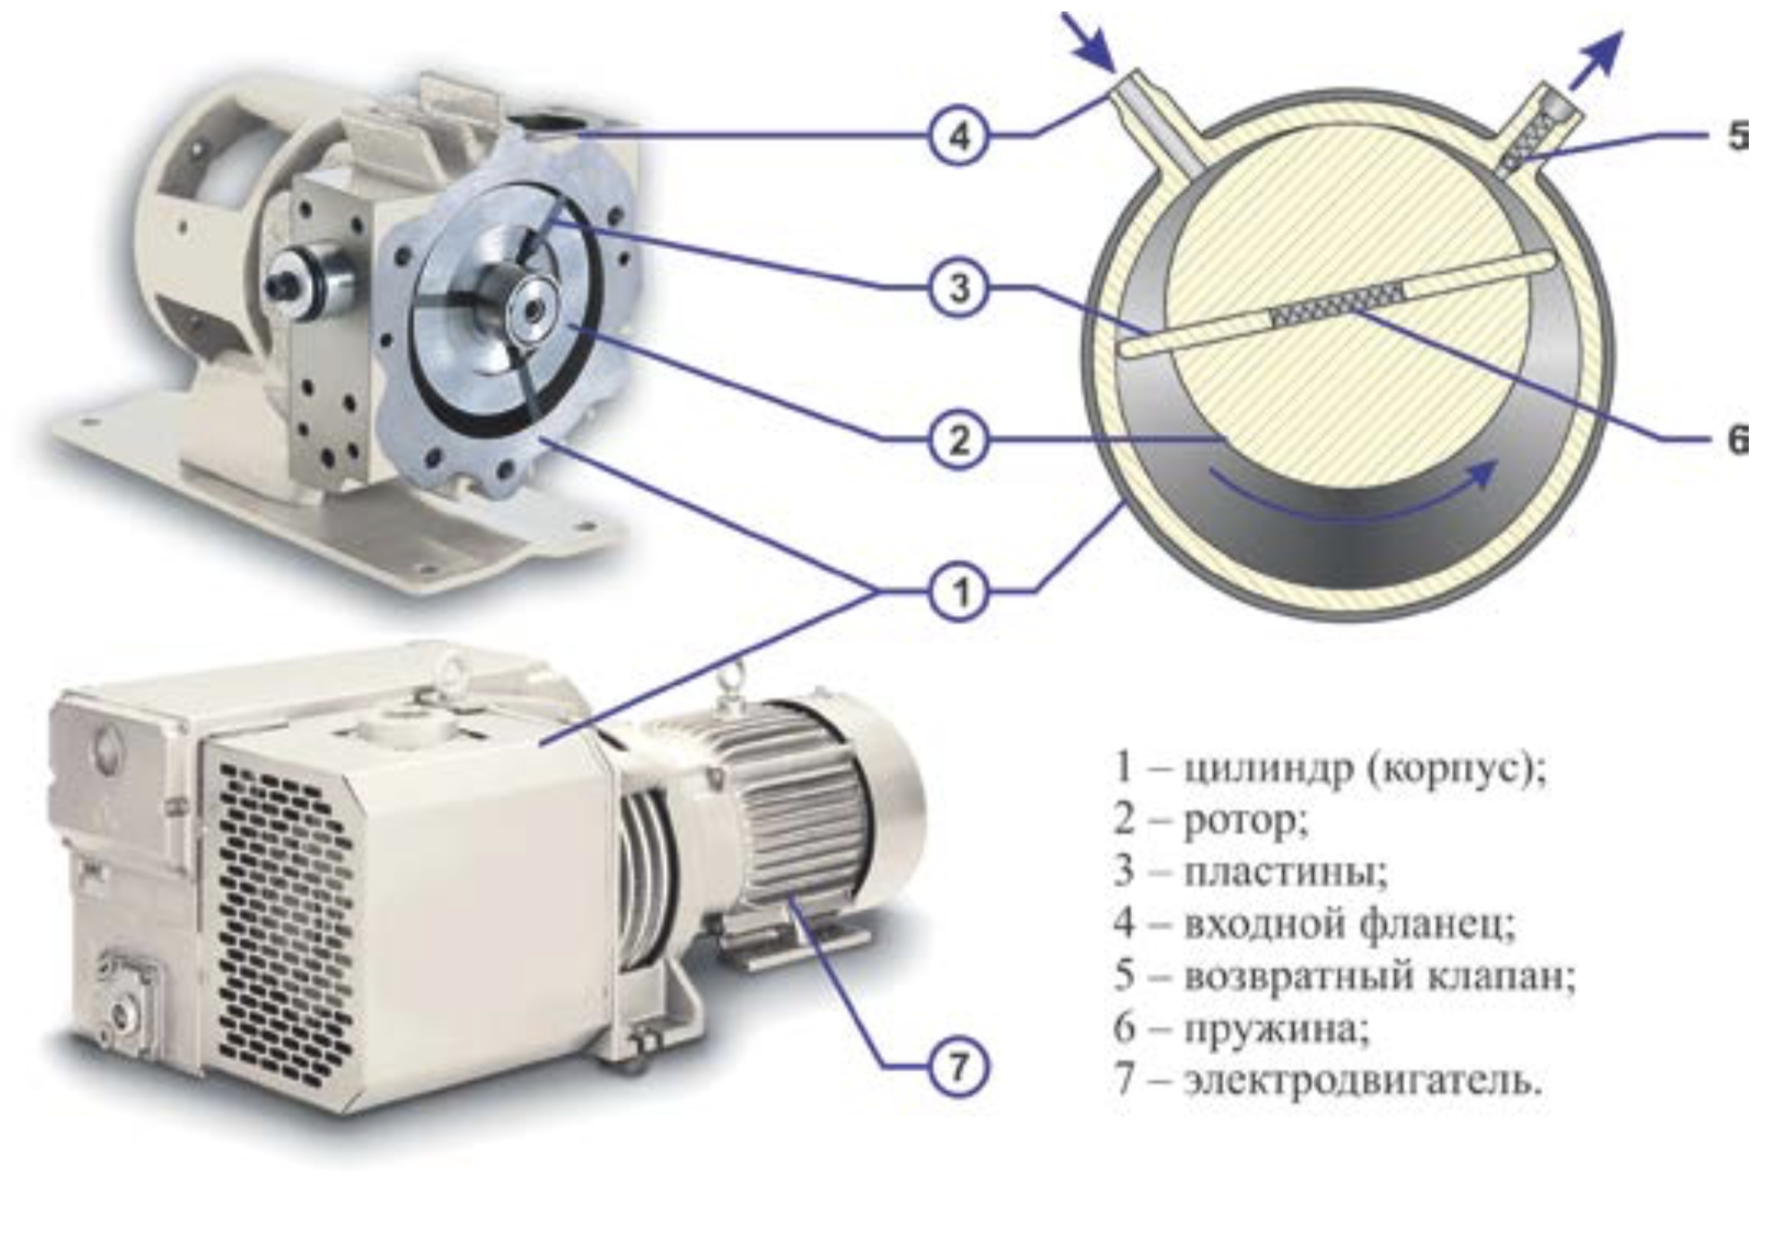
\includegraphics[width=0.6\linewidth]{2}
	\caption{Конструкция одноступенчатого пластинчато-роторного насоса}
	\end{center}
\end{figure}
\begin{itemize}
	\item Преимущества: неприхотлив в работе (может откачивать загрязненную среду, без ущерба для конструкционных элементов); используется для предварительной (форвакуумной откачки) в системах откачки с низкими требованиями по чистоте откачиваемого объема; используется до 2х последовательных ступеней.
	\item Недостатки: присутствие в рабочей камере масла, контактирующего с откачиваемой средой (возможно попадание паров в откачиваемый объем) и необходимость периодической его замены; низкий предельный вакуум за счет обратного потока воздуха через выпускные клапаны; малоэффективен для откачки влажных сред (необходимо использовать газобалластное устройство).
	\item Тип вакуума: средний.
\end{itemize}
\subsubsection{Турбомолекулярный насос}
Откачка в турбомолекулярном насосе (рис. 3) осуществляется за счет соударения частиц газа с быстродвижущимися турбинными лопатками дисков ротора (1) специальной геометрии, которые придают им дополнительный импульс в заданном направлении потока. Между дисками ротора находятся диски статора (2) с обратно обращенными лопатками, направляющие поток молекул на следующие диски турбины по оптимальной траектории, минимизируя обратный поток. Каждая пара пластин ротора-статора образует одну ступень. Насос состоит из нескольких ступеней расположенных последовательно, каждая последующая ступень имеет меньшие геометрические размеры, что при постоянном потоке газа приводит к постепенному повышению давления до выпускного форвакуумного. Скорость вращения ротора современных турбомолекулярных насосов достигает нескольких десятков тысяч оборотов в минуту.

\begin{figure}[H] \TopFloatBoxes
	\begin{floatrow}
		\ffigbox{\captionsetup{justification=centering}
			\caption{Конструкция турбомолекулярного насоса}}{
		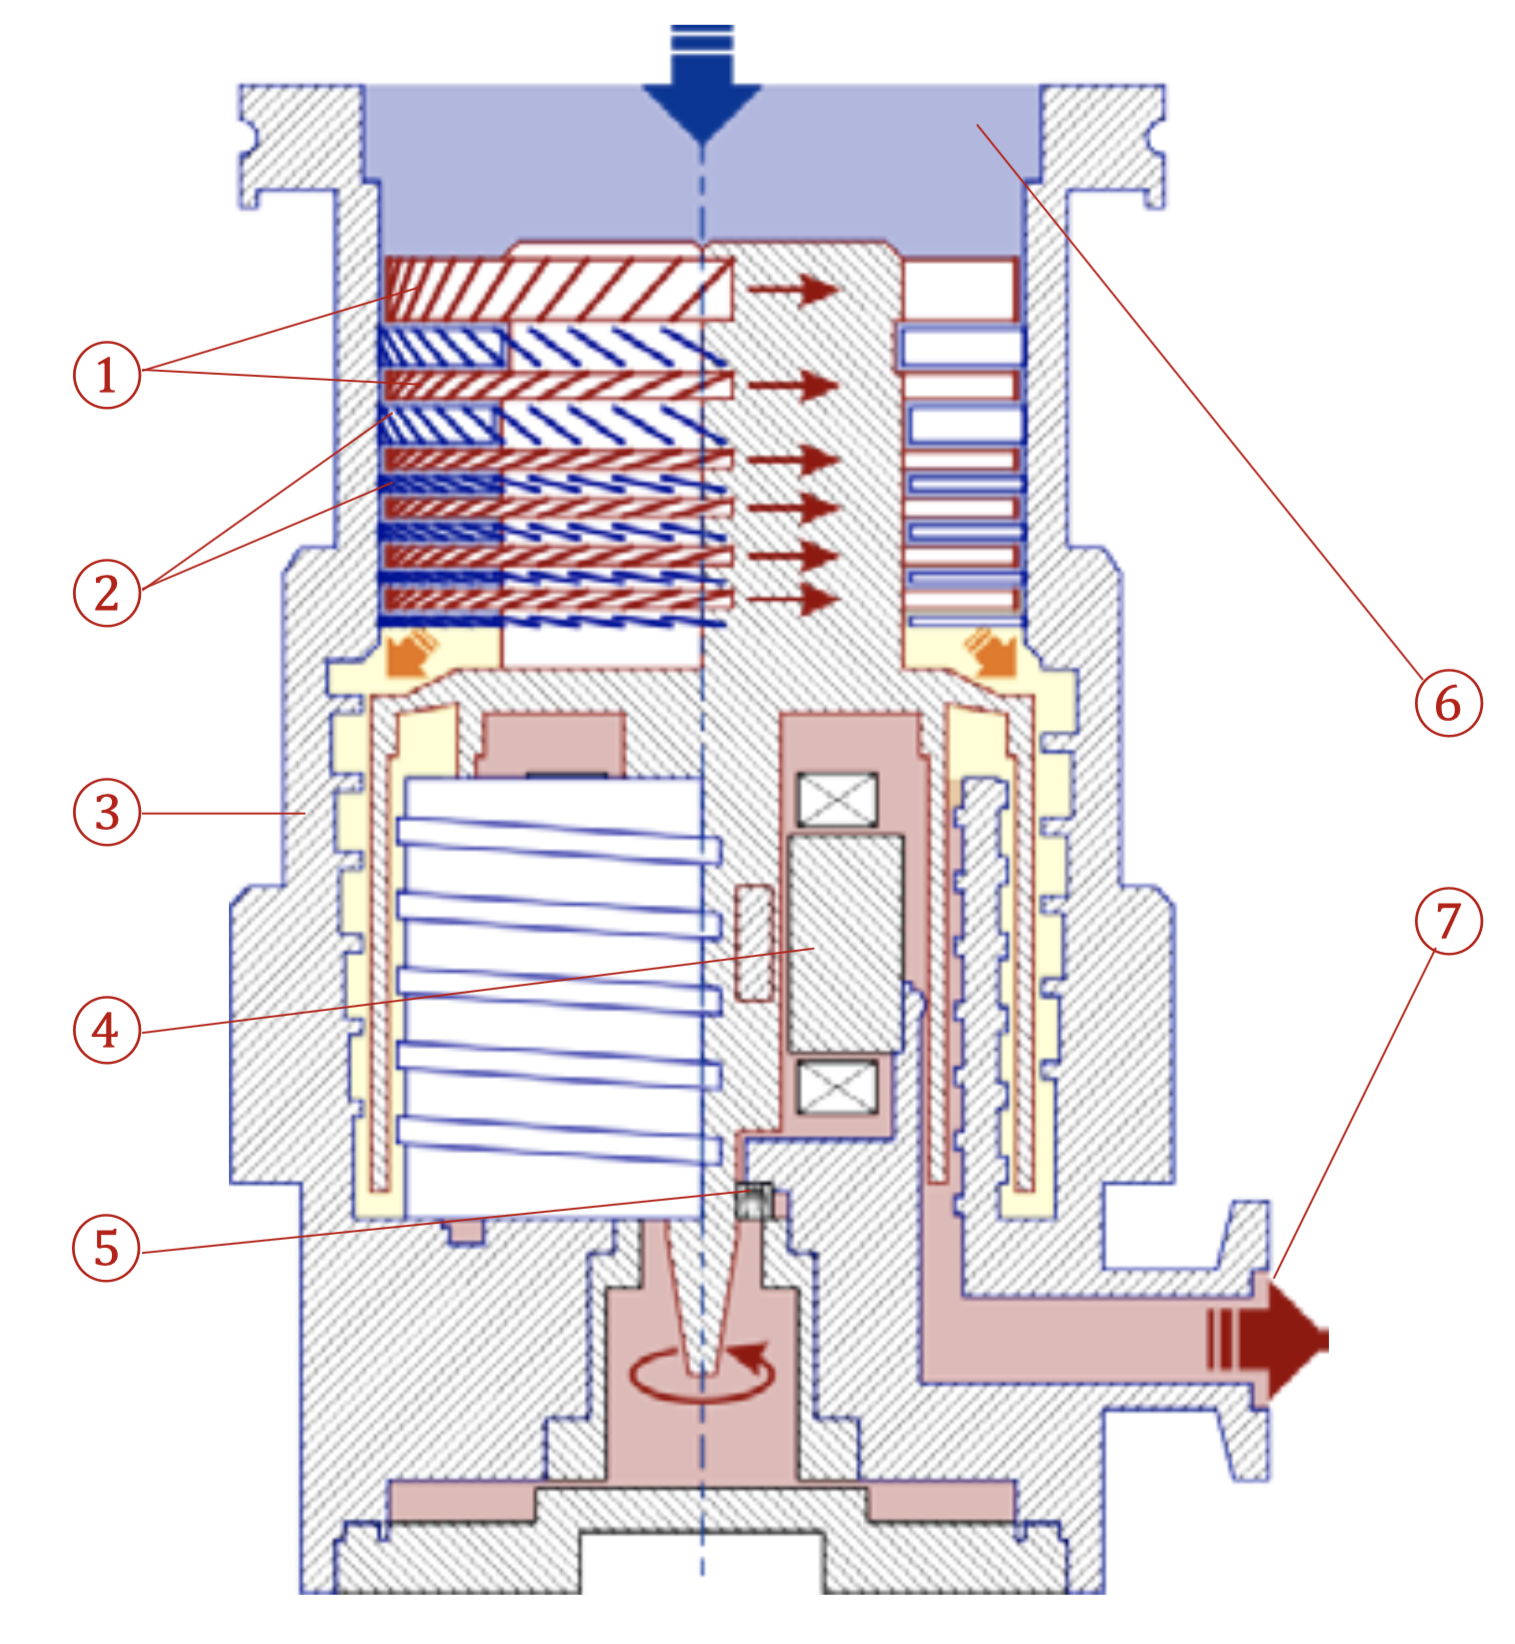
\includegraphics[width=\linewidth]{3}
	}
\killfloatstyle
\ttabbox{}{
	\begin{tabular}{p{0.4\linewidth}  p{0.4\linewidth}}
		\begin{enumerate}
			\item Ротор
			\item Статор
			\item Корпус насоса
			\item Электро-двигатель
			\item Нижний шарикоподшипник
		\end{enumerate}  &
		\begin{enumerate}
			\setcounter{enumi}{5}
			\item Высоко-вакуумный входной фланец
			\item Выпус-кной форвакуумный фланец
		\end{enumerate} 
	\end{tabular}
}
	\end{floatrow}
\end{figure}

\begin{itemize}
	\item Преимущества: постоянная готовность к работе; быстрый запуск ($\sim 10$ минут на раскручивание турбины); устойчивость к резкому повышению давления (вплоть до атмосферного); широкий диапазон рабочих давлений ($10^{-7} - 10^{-1}\text{Па}$); примерно одинаковая быстрота действия для большинства газов; используется как в системах <<сухой>> безмасляной откачки с особым требованием чистоты откачиваемого объема, так и с масляными форвакуумными насосами за счёт минимального обратного потока.
	\item Недостатки: требуется надежная защита вращающейся турбины от любых механических воздействий (пыли, абразивных частиц, вибраций, частых и резких перепадов давления и т. п.), приводящих к износу подвески ротора и разрушению лопаток турбины.
	\item Тип вакуума: высокий.
\end{itemize}
\subsection{Средства измерения вакуума}
\subsubsection{Терморезисторный вакуумметр (Пирани)}
Принцип действия тепловых манометров основан на зависимости теплопроводности газа от давления. Чувствительным элементом терморезисторного датчика (рис. 4) является тонкая металлическая нить накала (вольфрам, платина), помещенная в атмосферу откачиваемого газа. Сопротивление нити зависит от её температуры. Нить включена в одно из плеч мостовой схемы и разогрета до нескольких сотен градусов пропускаемым по ней током. Джоулево тепло, выделяемое нитью, отводится в основном через газовую среду со скоростью, зависящей от коэффициента теплопроводности. В зависимости от способа измерения вакуумметр работает в режиме (а) поддержания постоянного сопротивления моста (а значит и температуры нити), (б) постоянного напряжения на клеммах $А$, $С$ моста или (в) постоянного тока через мост. Мост изначально сбалансирован при давлении много ниже рабочего диапазона (сопротивление $R_\text{Б}$).

\begin{figure}[H]
	\begin{center}
		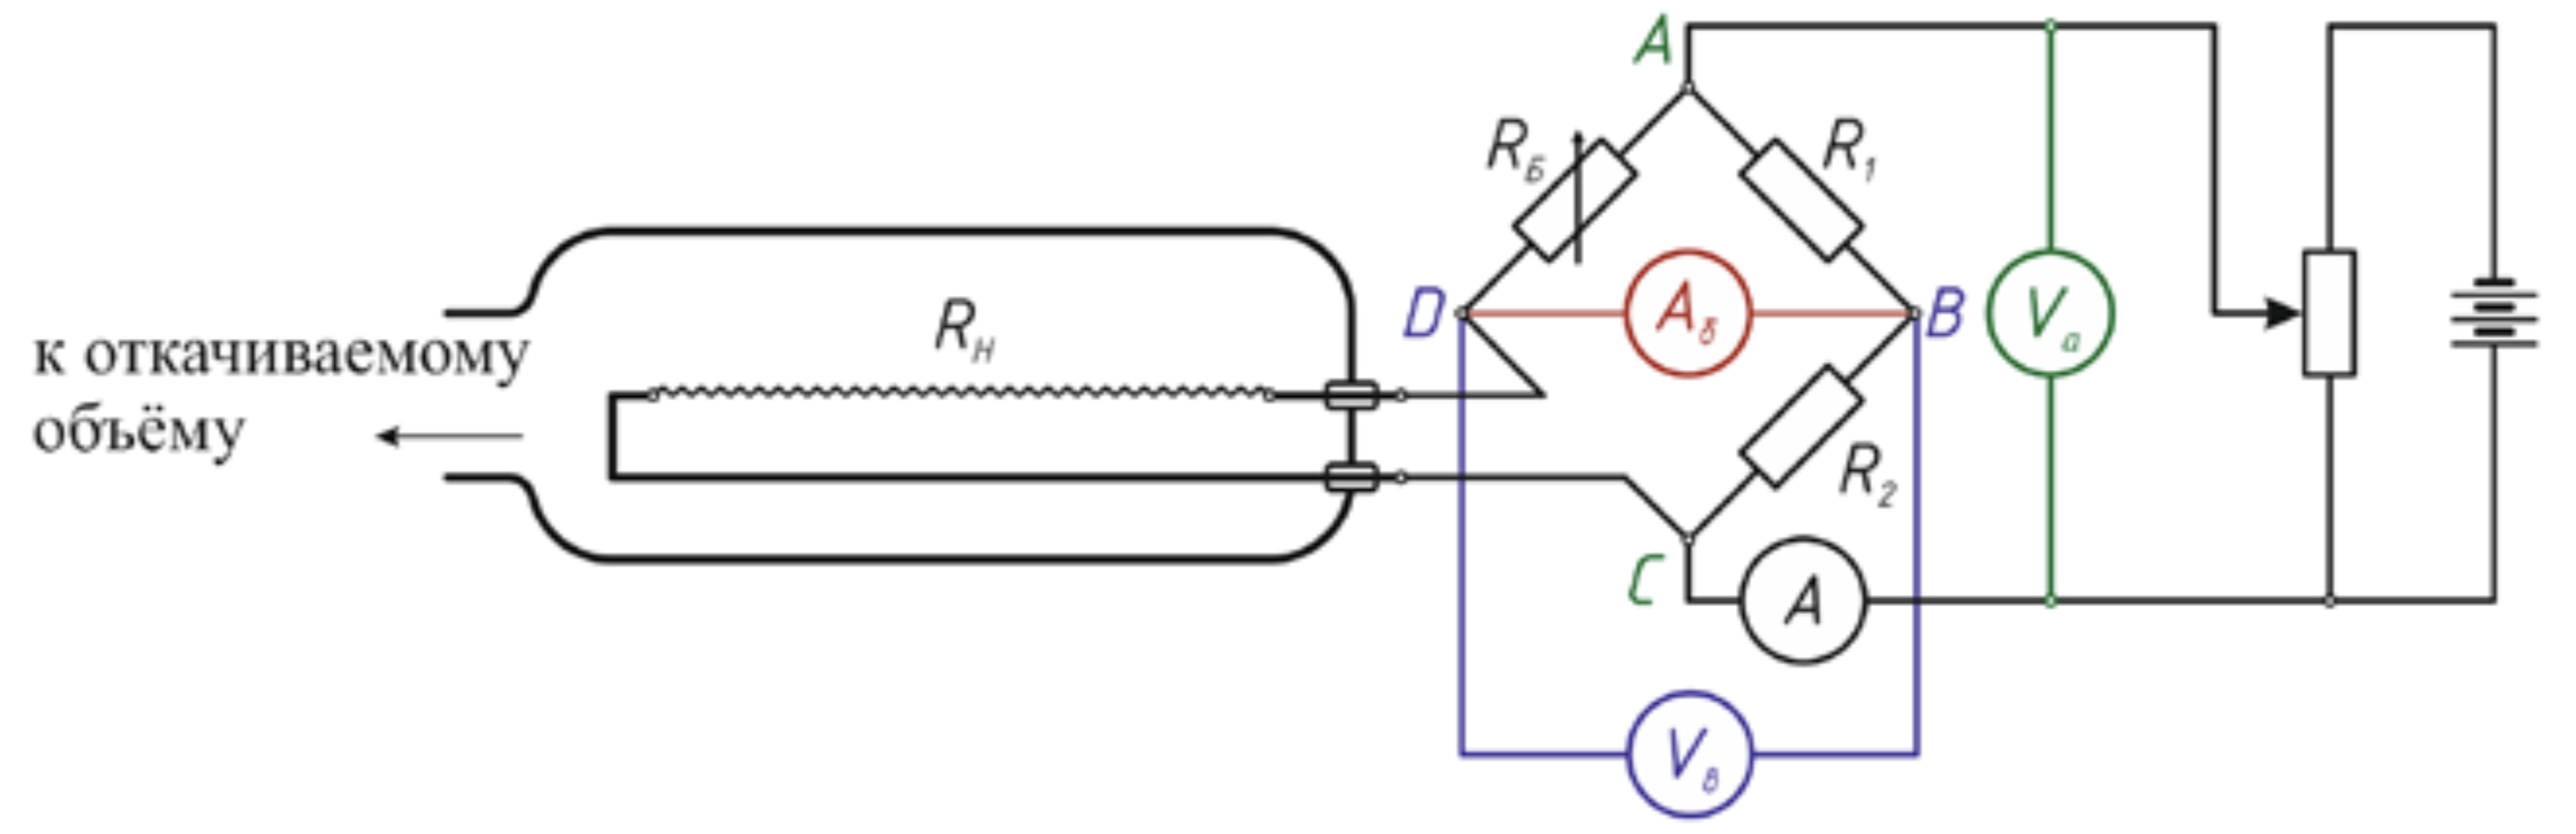
\includegraphics[width=\linewidth]{4}
		\begin{tabular}{p{0.4\linewidth} p{0.4\linewidth}}
			\begin{itemize}
				\item $R_\text{н}$ -- сопротивление нити накала
				\item $R_\text{б}$ -- сопротивление балансировки
				\item $V_\text{а}$ -- вольтметр для измерения напряжения на клемах $A$, $C$ в режиме (а)
			\end{itemize}  &
			\begin{itemize}
				\setcounter{enumi}{3}
				\item $A_\text{б}$ -- амперметр для измерения тока разбалансировки моста в режиме (б)
				\item $V_\text{в}$ -- вольтметр для измерения напряжения на клеммах 
			\end{itemize} 
		\end{tabular}
		\caption {Принципиальная схема терморезисторного вакуумметра (Пирани) }
	\end{center}
\end{figure}

В первом случае (а) напряжение на клеммах $А$, $С$ моста автоматически подбирается так, чтобы мост всё время оставался сбалансированным при изменении давления и, тем самым, является мерой давления в системе:
\[P\sim V^2 -V_0^2 \]
где $V_0$ -- напряжение на клемах при начальной балансировке.

Во втором случае (б) мерой давления служит ток разбалансировки моста, в третьем (в) — напряжение на клеммах $B$, $D$.

В области низкого вакуума при $\lambda \gg d$ коэффициент теплопроводности перестаёт зависеть от давления, а при давлениях менее $10^{-3}\ \text{Торр}$ основную роль в процессе теплоотвода начинает играть излучение. Оба эти фактора ограничивают применение данного типа датчиков областью среднего вакуума.

\begin{itemize}
	\item Преимущества: Практически неограниченный срок службы в неагрессивных средах за счёт низкой степени окисления нити при низких температурах нагрева. Способность выдержать прорыв атмосферы.
	\item Недостатки: при давлениях более $1\text{мбар}$ показания существенно зависят от типа газа; тепловая инерция — запаздывание показаний при резком изменении давления; необходимость перекалибровки датчика в связи с изменением сопротивления после длительного времени эксплуатации.
	\item Тип вакуума: средний.
\end{itemize}
\subsubsection{Магнетронный вакуумметр (с холодным катодом)}
Случайным образом возникшие вблизи катода электроны (например, вследствие автоэлектронной эмиссии ) будут двигаться к аноду под действием скрещенных электромагнитных полей по удлиненной траектории. При этом повышается вероятность соударения электронов с молекулами откачиваемого газа и их ионизация. Образовавшиеся ионы ускоряются в электрическом поле анодно-катодного промежутка и выбивают из материала катода вторичные электроны (вторичная электронная эмиссия), которые также ионизируют газ, двигаясь к аноду по сложной циклической траектории.

\begin{figure}[H]
	\begin{center}
		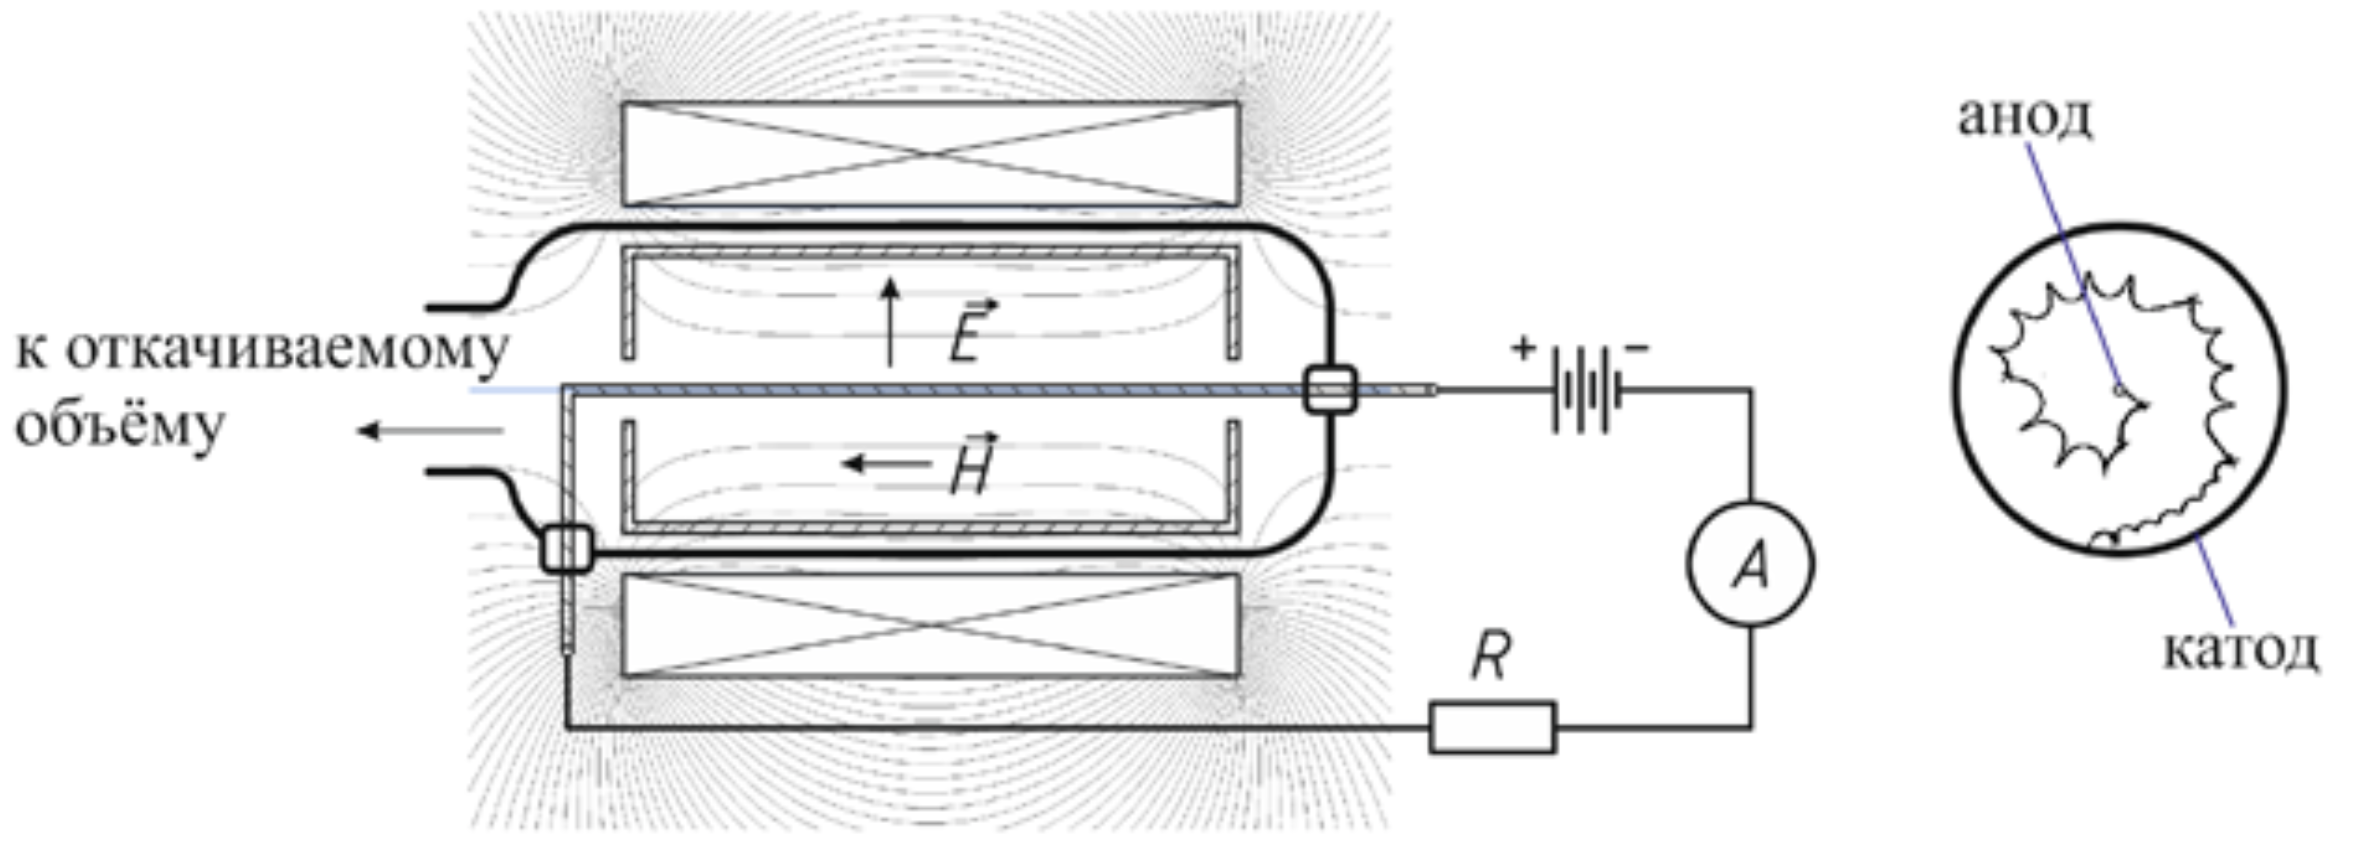
\includegraphics[width=\linewidth]{5}
		\captionsetup{justification=centering}
		\caption{Принципиальная схема инверсно-магнетронного вакуумметра и траектории электронов в них}
	\end{center}
\end{figure}

В результате описанного процесса возникает электрический разряд, ток которого в достаточно широком диапазоне зависит от давления. На диапазон измеряемых давлений существенно влияет конструкция магнетронного датчика. В инверсно-магнетроном датчике анодом служит центральный металлический стержень, а катодом — осесимметричная обечайка, магнитное поле создается внешним постоянным кольцевым магнитом (рис. 5).
\begin{itemize}
	\item Преимущества: Могут включаться в широком диапазоне давлений, т.к. не содержат накаленных деталей и не боятся окисления. Устойчивы к прорыву атмосферы. Применяются в автоматизированных технологических процессах вследствие простоты эксплуатации и нечувствительности к внешним воздействиям.
	\item Недостатки: Не желательно длительное использование в диапазоне среднего вакуума особенно в атмосфере аргона, т.к. это приводит к распылению материала катода потоком ионов, что, в свою очередь, может стать причиной короткого замыкания и сбоев датчика. Не желательно использование в системах с масляным типом откачки, т.к. углеводороды со временем образуют устойчивую пленку на поверхности катода, которая искажает показания датчика. Является источником магнитного поля, что может влиять на работу других приборов.
	\item Тип вакуума: высокий, сверхвысокий.
\end{itemize}
\subsubsection{Термоэлектронный вакууметр}
Катодом термоэлектронного вакуумметра является накаливаемая нить (1) (\mbox{рис. 6}). 
\begin{figure}[H]
	\begin{center}
		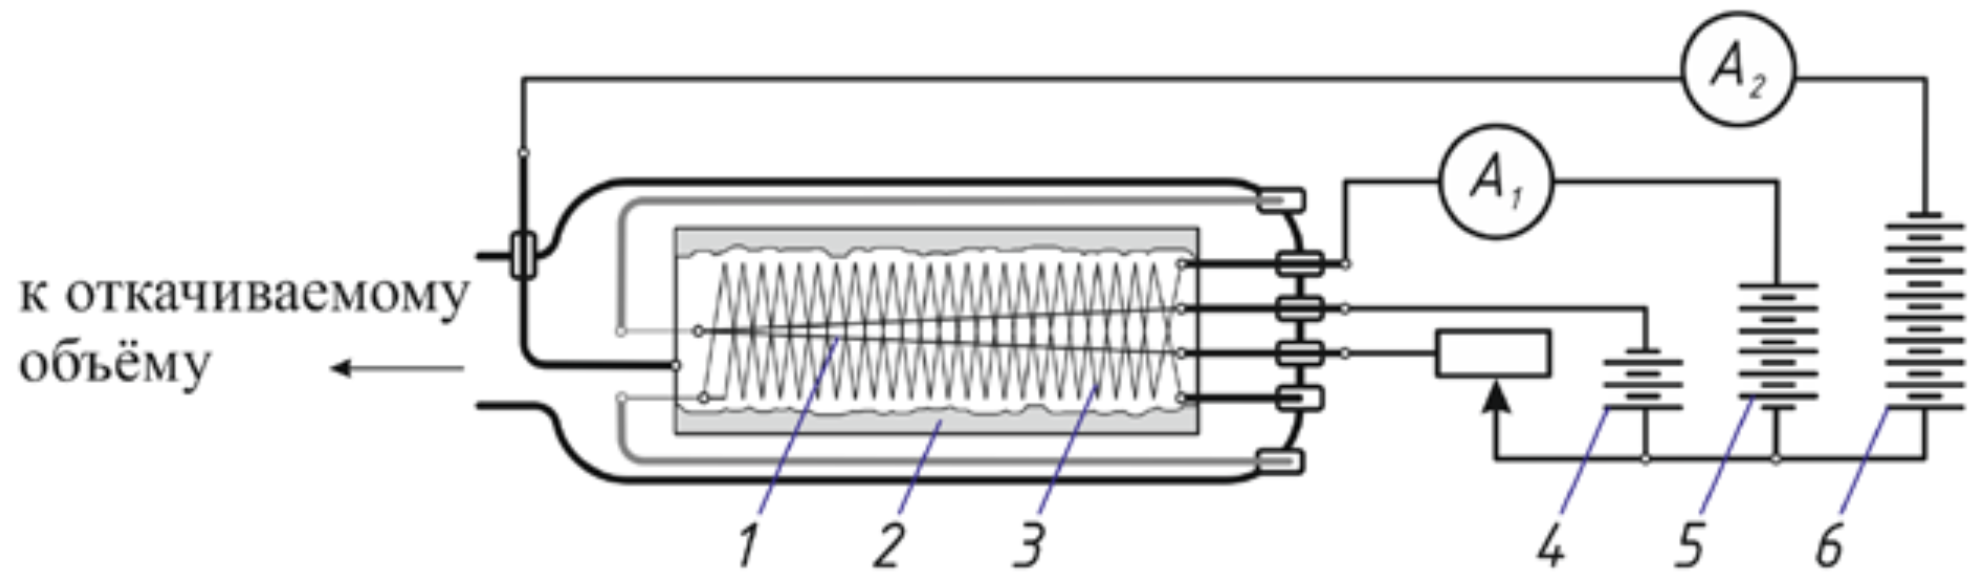
\includegraphics[width=\linewidth]{6}
		\begin{tabular}{p{0.5\linewidth} p{0.45\linewidth}}
			\begin{enumerate}
				\item Катод
				\item Коллектор
				\item Анод
				\item Цепь регулировки тока накала
				\item Цепь анода
			\end{enumerate}  &
			\begin{enumerate}
				\setcounter{enumi}{5}
				\item Цепь коллектора
				\item $A_1$ -- амперметр для измерения электронного тока
				\item $A_2$ -- амперметр для измерения ионного тока
			\end{enumerate} 
		\end{tabular}
		\caption {Принципиальная схема термоэлектронного вакууметра}
	\end{center}
\end{figure}

Эмитируемые накаленным катодом электроны под действием ускоряющего электрического поля устремляются по направлению к аноду (2), создавая в его цепи (5) электронный ток. Анод, как правило, выполнен в виде спирали или сетки с большим шагом, поэтому значительная часть электронов проходит между витками анода и тормозится полем коллектора 3, имеющего по отношению к катоду отрицательный потенциал. Не дойдя до коллектора ионов, электроны останавливаются и начинают движение обратно к аноду-сетке. Снова значительная часть электронов проходит между витками анода и тормозится уже полем катода. Каждый электрон может сделать несколько таких колебаний, прежде чем попасть на сетку.
\begin{itemize}
	\item Преимущества: применимость для измерения давлений всех газов и паров.
	\item Недостатки: зависимость показаний от рода газов; необходимость обезгаживания для устранения искажения показаний, недопустимость работы выше заданного диапазона давлений и прорыва атмосферы при включенном катоде (накаленная спираль быстро окисляется и перегорает).
	\item Тип вакуума: высокий.
\end{itemize}
\subsection{Экспериментальная установка}
Схема экспериментальной установки представлена на рис. 7
\begin{figure}[H]
	\begin{center}
		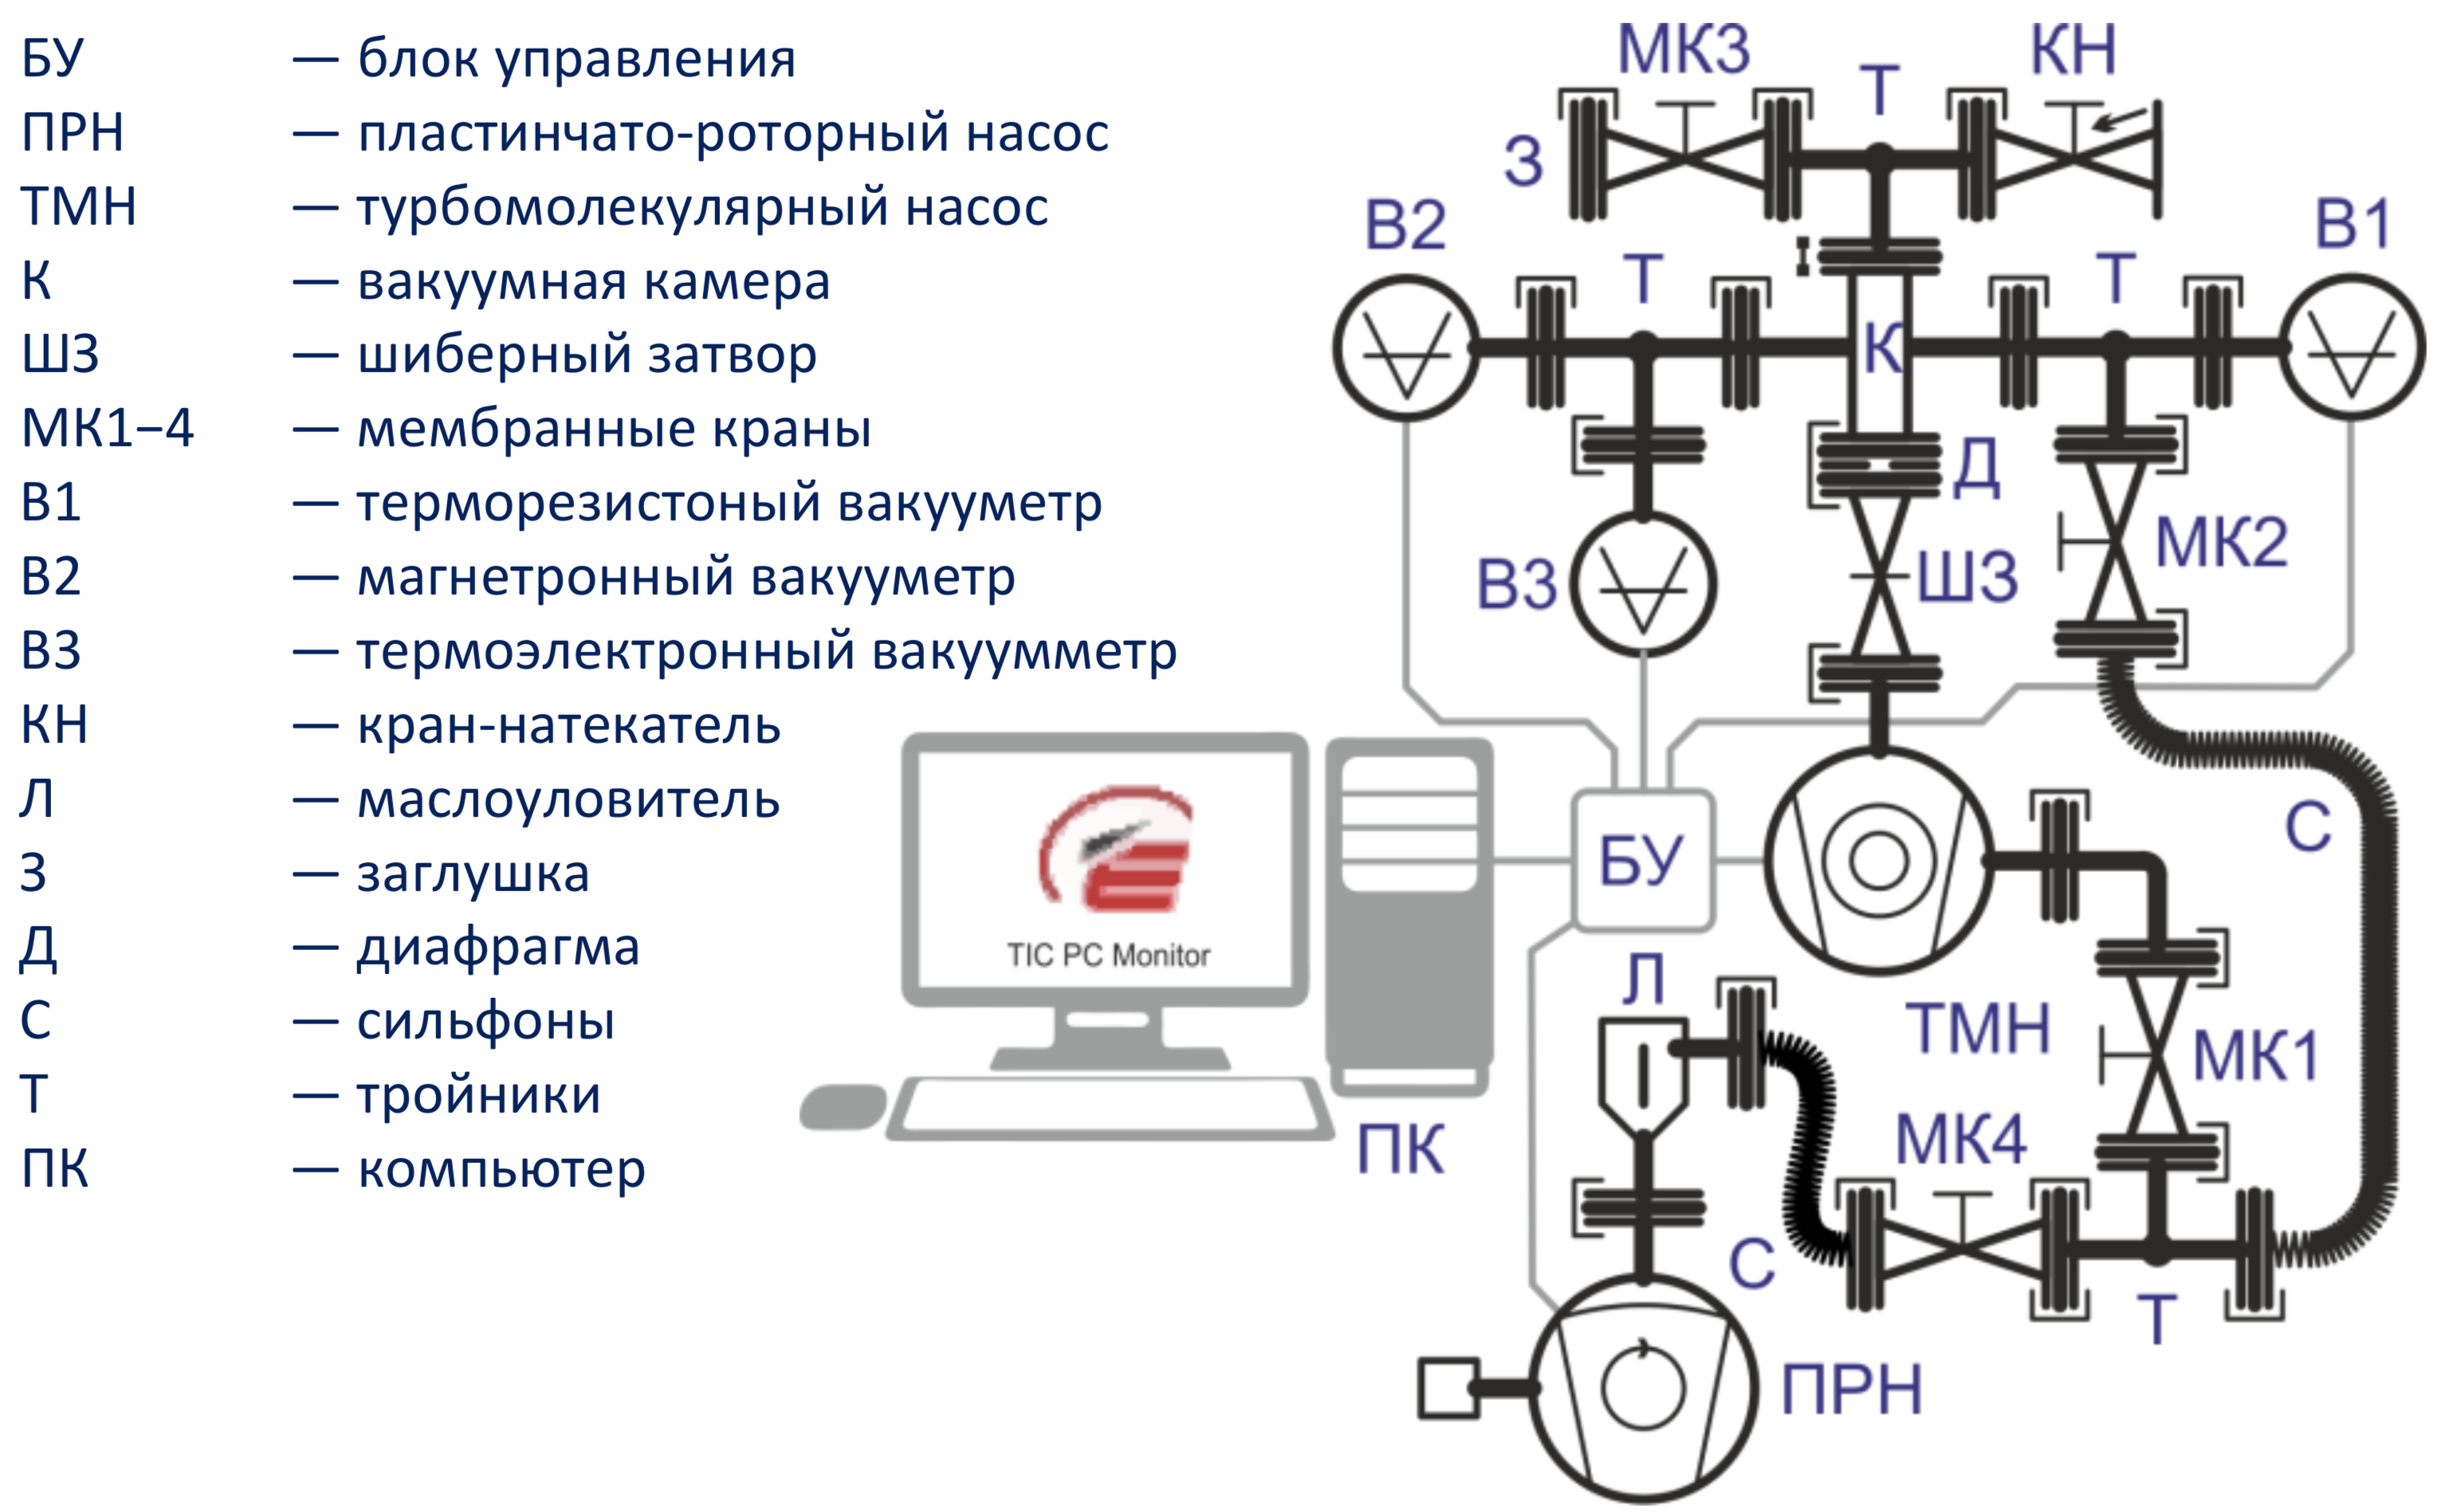
\includegraphics[width=\linewidth]{7}
		\caption{Схема экспериментального стенда}
	\end{center}
\end{figure}
\section{Результаты измерений и обработка результатов}
\subsection{Определение объемов различных частей установки}
При закрытии в откачанной установке крана $MK2$ и последующим открытием крана $MK3$ воздух из сильфона поступает в вакуумную камеру и прилежащие к ней вакууметры. При этом показания вакуумметров резко увеличатся. Воспользуемся законом Бойля-Марийотта для нахождения объема камеры $K$.
\[P_0V_0 = P_1(V_0 +V_\text{к})\]
где $P_0$ -- начальное давление в системе, $V_0$ -- объем сильфона, $P_1$ -- давление в системе после открытия $MK3$, a $V_\text{к}$ -- объем камеры. Отсюда
\begin{align*}
\begin{aligned}
V_\text{к} = \frac{P_0 - P_1}{P_1}V_0, & &\Delta V_\text{к}= \frac{P_0V_0}{P_1^2}\Delta P_1
\end{aligned}
\end{align*}
\begin{figure}[H]
	\begin{center}
		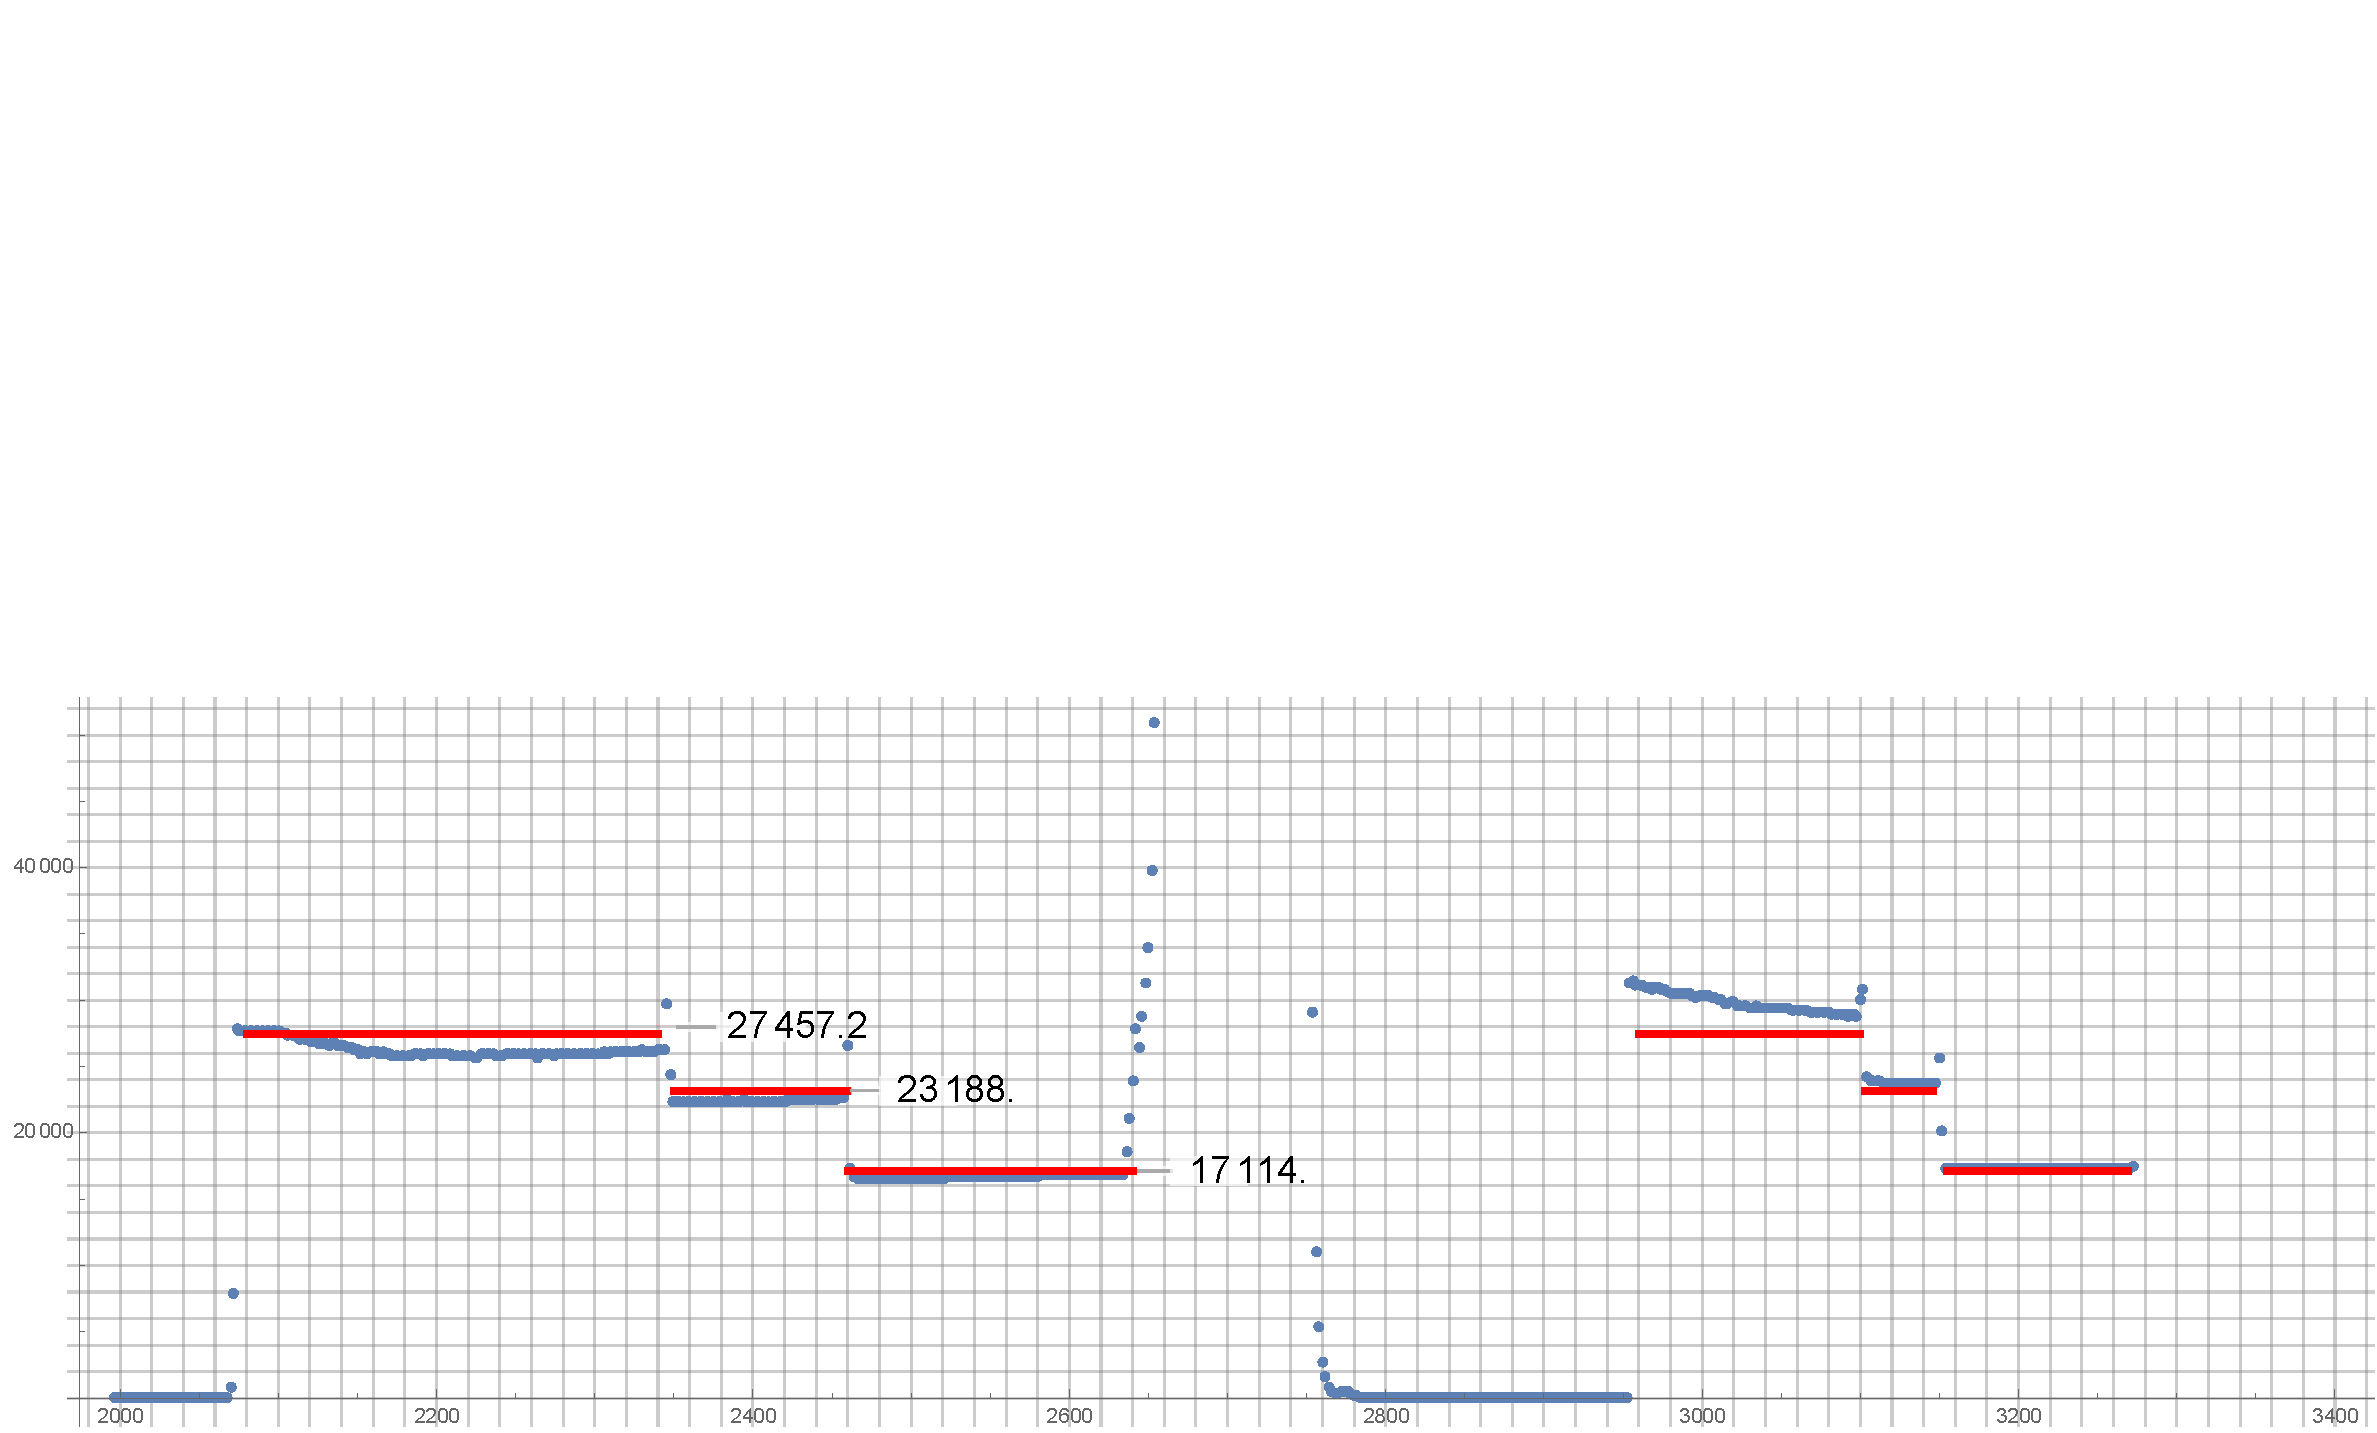
\includegraphics[width=\linewidth]{11}
		\caption{График зависимости $P(t)$ при открытии кранов}
	\end{center}
\end{figure}
Из графика на рис. 8 получаем 
\[P_1 = (27,5 \pm 1,8)\ \text{кПа}\]
\[V_\text{к} = (664 \pm 43)\ \text{мл}\]
Аналогично по графику определяются объем $V_\text{c}$ форвакуумной магистрали, объем $V_\text{н}$ насоса ТМН и объем $V$ всей установки
\begin{align*}
V_\text{c} &= \frac{P_0 - P_2}{P_2}V_0-V_\text{к}\\
V_\text{н} &= \frac{P_0 - P_3}{P_3}V_0-V_\text{к} - V_\text{с}\\
V &= \frac{P_0 - P_3}{P_3}V_0
\end{align*}
где $P_2 = (23,2 \pm 1,7)\ \text{кПа}$ -- давление в системе после открытия крана $MK2$,\\ $P_3=(17,1\pm 1,1)\text{кПа}$ -- давление в системе после открытия крана $MK1$. 

\noindent Таким образом
\begin{align*}
V_\text{c} &= (170 \pm 17)\ \text{мл}\\
V_\text{н} &= (388\pm 52)\ \text{мл} \\
V &= (1222 \pm 79)\ \text{мл}
\end{align*}
\subsection{Оценка скорости натекания}
При работе с высоким вакуумом, создаваемым TМН, скорость натекания воздуха сравнима со скоростью откачки. Исходя из уравнения (5), после закрытия шиберного затвора откачка воздуха из камеры $K$ прекращается и зависимость давления в системе от времени должна иметь вид
\[ P(t) = P + \frac{Q_\text{н}}{V_\text{к}}t\]
\begin{figure}[H]
	\begin{center}
		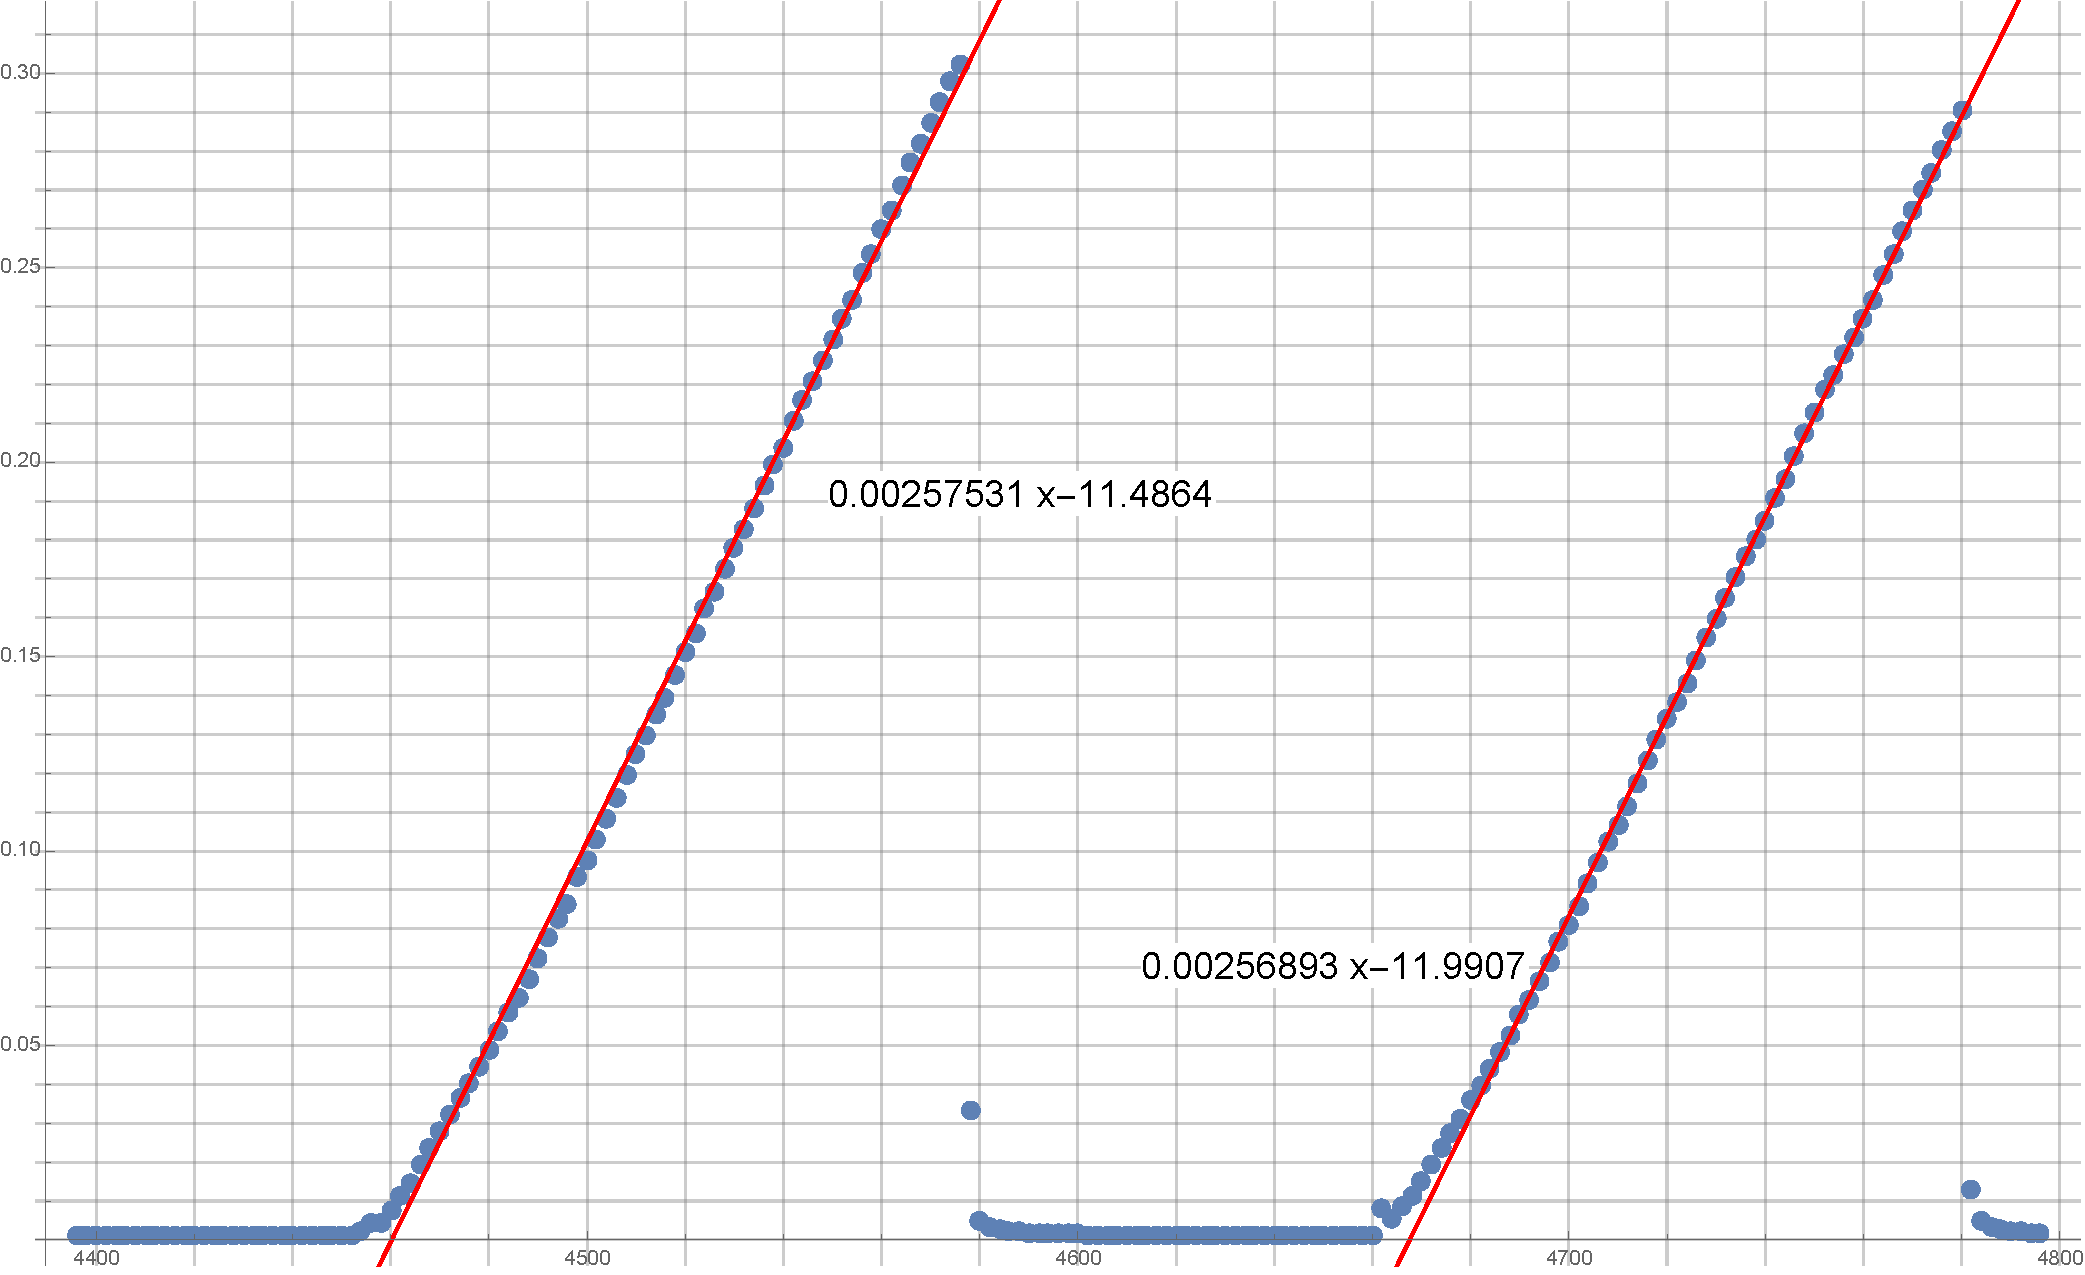
\includegraphics[width=\linewidth]{12}
		\caption{Зависимость $P(t)$ при открывании шибера}
	\end{center}
\end{figure}
Из графика на рис. 9 получаем:
\[Q_\text{н} = (1,7\pm0,1)\cdot10^{-6}\ \text{Па}\cdot \text{л}/\text{с}\]

\subsection{Оценка числа Кнудсена и определение эффективной скорости откачки ПРН}
зависимость длины свободного пробега молекул от давления при постоянной температуре имеет вид $\lambda \sim 1/р$. Поэтому при давлении $P$ в системе длина свободного пробега молекул равна
\[\lambda = \frac{P_0}{P}\lambda_0\]
где $P_0$ - атмосферное давление, а $\lambda_0$ - длина свободного пробега молекул при атмосферном давлении ($\lambda_0 \sim 0,7 \cdot 10^{-6} \text{см}$). Указанный в инструкции характерный размер проводящих частей установки равен $r \sim 11 \text{мм}$. Таким образом в диапазоне давлений $1 \div 10 \text{кПа}$ $\lambda_1 \approx10^{-4} \text{см}$ и ${Kn}_1 \approx 10^{-4} \ll 1$, что соответствует вязкостному режиму, а в диапазоне давлений $10 \div 100 \text{Па}$ $\lambda_2 \approx 10^{-1} \text{см}$ и ${Kn}_2 \approx 0,1 \sim 1$, что соответствует переходному режиму. При работе с высоким вакуумом (насос ТМН) число Кнудсена становится приблизительно равным $20$, что уже может соответствовать Кнудсеновскому режиму, однако данный диапозон давлений малоинтересен для изучения ввиду сравнительно большой для него скорости натекания (нарушается условие (7)).

Данный переход от одного режима откачки к другому можно наблюдать на графике зависимости $\ln P(t)$ при работе насоса ПРН. При давлении в системе $p \sim 10000\ \text{Па}$ скорость движения воздуха по трубкам имеет порядок $\upsilon  \sim 1 \text{м}/\text{с}$, его плотность $\rho sim 0,1 \text{кг}/\text{м}^3$, длина трубок $L \approx 0, 5 \text{м}$, а вязкость воздуха $
\eta \approx 20\cdot 10^{-6}\ \text{Па}$. При таких оценочных значений параметров число Рейнольдса для движения воздуха имеет значение $Re \sim 2500$, чего вполне достаточно, чтобы считать течение воздуха ламинарным. Значит, применение формулы Пуазейля допустимо, из чего следует справедливость формулы (12). Подставляя в нее все характерные значения, получим, что
\[U_\text{н} \approx 6 \text{л}/\text{с}\]
что говорит о незначительном влиянии воздуха на проводимость системы.

Построим график зависимости $\ln P(t)$ для ПРН.
\begin{figure}[H]
	\begin{center}
		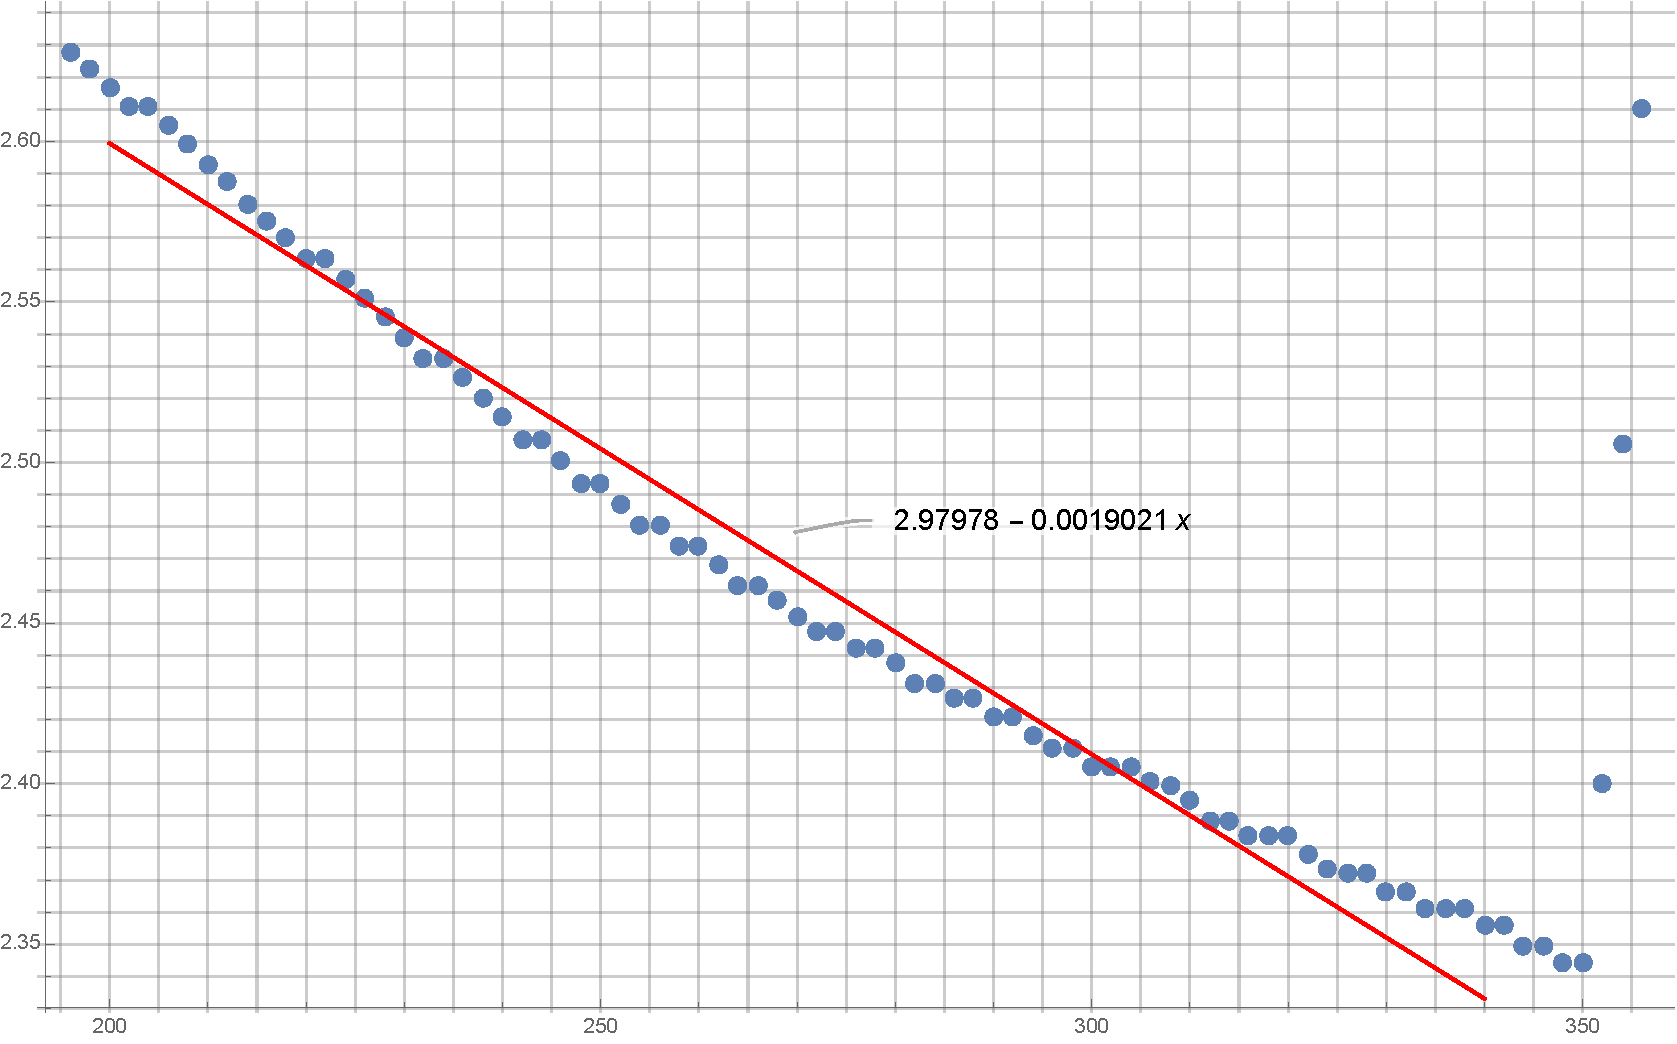
\includegraphics[width=0.9\linewidth]{13}
		\caption{Зависимость $\ln P(t)$ для ПРН насоса}
	\end{center}
\end{figure}
Из графика на рис. 10 получаем:
\begin{align*}
\tau_1 &= (500 \pm 15) \text{с}\\
S_{01} &= (1,3\pm 0,1) \text{мл}/\text{c}
\end{align*}

Построим график зависимости $\ln P(t)$ для ТМН.
\begin{figure}[H]
	\begin{center}
		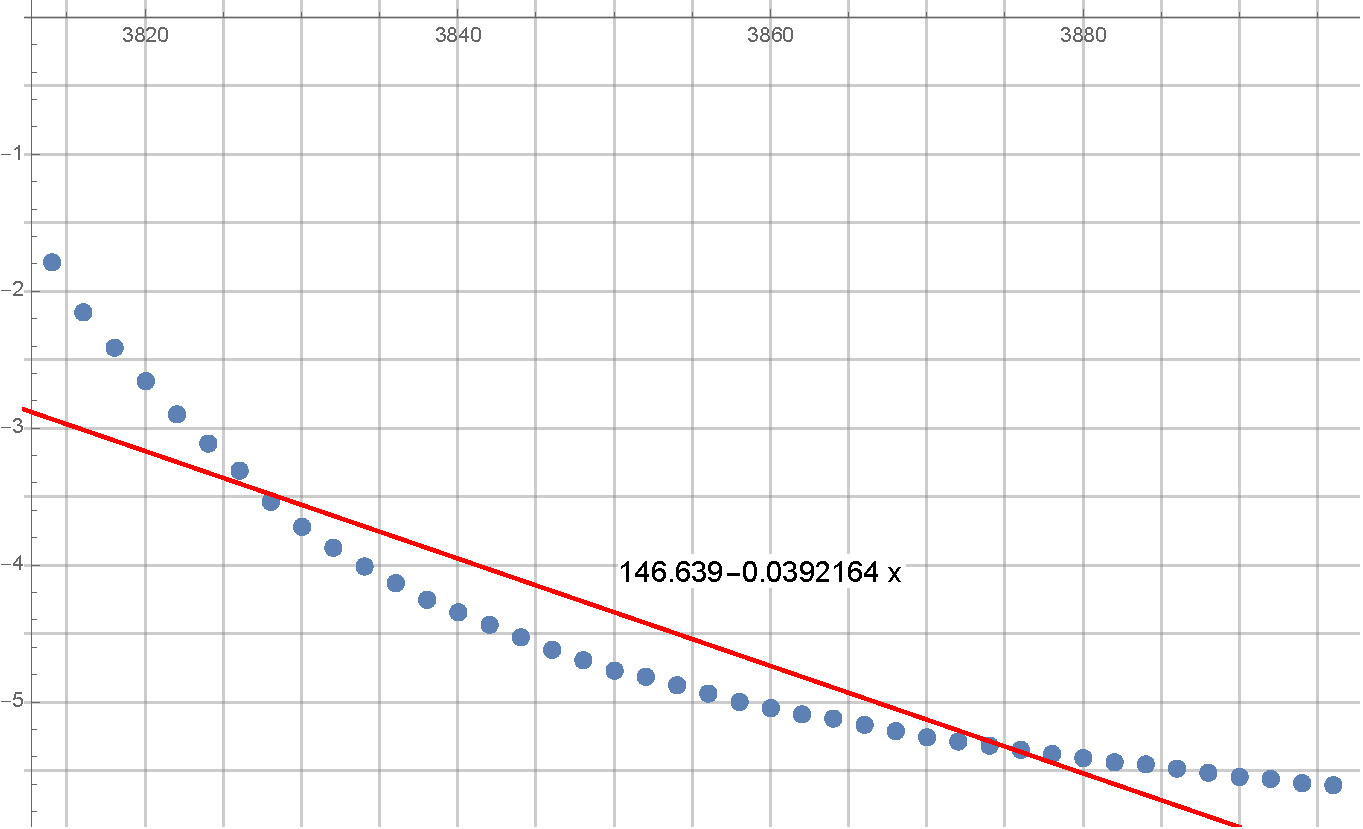
\includegraphics[width=0.9\linewidth]{14}
		\caption{Зависимость $\ln P(t)$ для ТМН насоса}
	\end{center}
\end{figure}
Из графика на рис. 11 получаем:
\begin{align*}
\tau_2 &= (25 \pm 2) \text{с}\\
S_{02} &= (26\pm 3) \text{мл}/\text{c}
\end{align*}
\section{Обсуждение результатов и выводы}
В работе были измерены: объем крана $V_\text{к}$, объем форвакуумной магистрали $V_\text{с}$, объем насоса (ТМН) $V_\text{н}$ и объем всей установки $V$
\begin{align*}
V_\text{к} &= (664 \pm 43)\ \text{мл}\\
V_\text{c} &= (170 \pm 17)\ \text{мл}\\
V_\text{н} &= (388\pm 52)\ \text{мл} \\
V &= (1222 \pm 79)\ \text{мл}
\end{align*}
Была проведена оценка скорости натекания для ТМН:
\[Q_\text{н} = (1,7\pm0,1)\cdot10^{-6}\ \text{Па}\cdot \text{л}/\text{с}\]
Также было посчитано время откачки $\tau$ и скорость откачки $S_0$ для ПРН и ТМН.
\begin{align*}
\tau_1 &= (500 \pm 15) \text{с}\\
S_{01} &= (1,3\pm 0,1) \text{мл}/\text{c}\\
\tau_2 &= (25 \pm 2) \text{с}\\
S_{02} &= (26\pm 3) \text{мл}/\text{c}
\end{align*}
\end{document}